\chapter{Design}
\label{ch_design}

This chapter is dedicated to the various modules which comprise the laser tag system being investigated. The system is complex and comprises of many modules both in hardware and software. An overview of the entire system is given followed by the design of the individual modules.

The system overview covers the two main subsystems, the tagger subsystem and target subsystem. Following the system overview these two subsystems are divided into modules and categorized into either hardware or software. The design of each module is presented, along with an image of the final implementation.

%todo: possibly explain why designs are so ellaborate... This investigation is centred on the creation and evaluation of system modules, therefore the design descriptions have been written 

%todo: give an explaination as to how the module design has been brocken down into subsubsections

\section{System Overview}

Figure \ref{fig:system_overview_hardware} gives an overview of the modules that make up the laser tag data link system.

\begin{figure}[H]
	\centering
	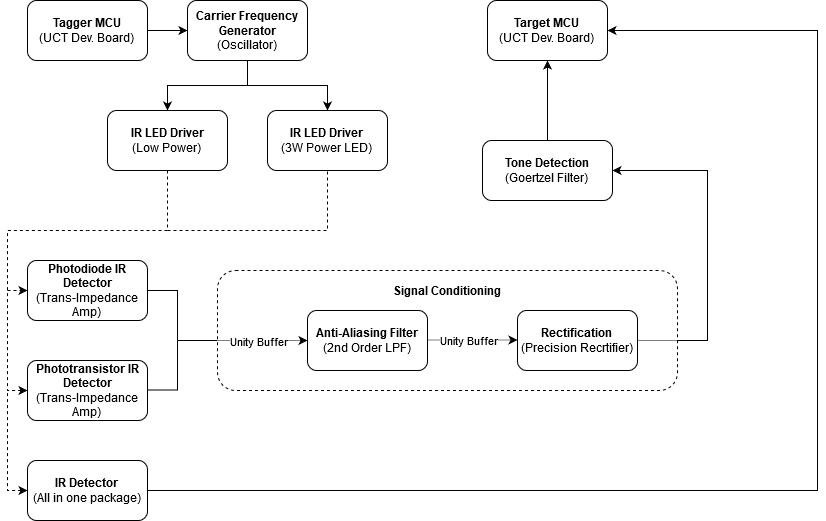
\includegraphics[width=0.9\textwidth]{figures/design/system_overview_hardware}
	\caption{Block Diagram of Hardware Modules}
	\label{fig:system_overview_hardware}
\end{figure}

\subsection{Subsystems}

Two subsystems may be derived from figure \ref{fig:system_overview_hardware}. The tagger subsystem responsible for generating and transmitting a message and the target subsystem responsible for receiving and decoding an incoming message.

\subsubsection{Tagger Subsystem}
The tagger subsystem comprises a main processor, carrier frequency generation module and two LED driver modules. For the purposes of this investigation the UCT STM32\footnotemark{} development board has been used as the main processor. The development board communicates with the carrier frequency generation module (responsible for producing the 36kHz square waveform), this module is connected to an LED driver module which in turn drives an IR LED. Two led driver modules have been design and both operate on the same input signal. The difference between the two modules is in the rated output power, the low power module is designed to drive a standard low power IR led while the high power module has been designed to drive a high power 3W IR led.

Not shown on the system overview is the light focus hardware module. This module is a passive optical component designed to focus the IR light.

\footnotetext{STM32F051C6}

\subsubsection{Target Subsystem}
The target system comprises more modules than the tagger due to the comparably higher complexity involved in detecting and processing incoming signals. The first stage of this subsystem concerns detecting incoming IR light, three different modules have been designed to perform this operation to allow for comparison between these separate approaches. As outlined in the overview shown in figure \ref{fig:system_overview_hardware} the IR receiver demodulates the detected IR light directly, however the remaining two detectors required additional modules to condition and demodulate the Manchester sequence.

These additional modules perform anti-alias filtering and rectification of the signal as well as indicate when a 36kHz tone is present in the conditioned signal. This tone detection is performed by a digital signal processing (DSP) algorithm and is implemented on the STM32 MPU.

The final module of the target subsystem is the main processor which is implemented on a second UCT STM32 development board.

\subsubsection{Software}

There are three main software components to the overall system.
\begin{itemize}
	\item The software operating on the tagger main processor used to encode and produce the Manchester data sequence.
	\item The software responsible for receiving and decoding the Manchester sequence on the target main processor.
	\item  The DSP algorithm operating on the tone detection module.
\end{itemize}


\section{Hardware Design}

\subsection{Tagger \& Target MCUs}
%Missing
% - Schematic and the like in the appendix
The laser tag systems has two main processors. One for the tagger and another for the target. The hardware used for main processor in each case is the UCT development board built around the STM32F051C6 microcontroller.

\begin{figure}[H]
	\centering
	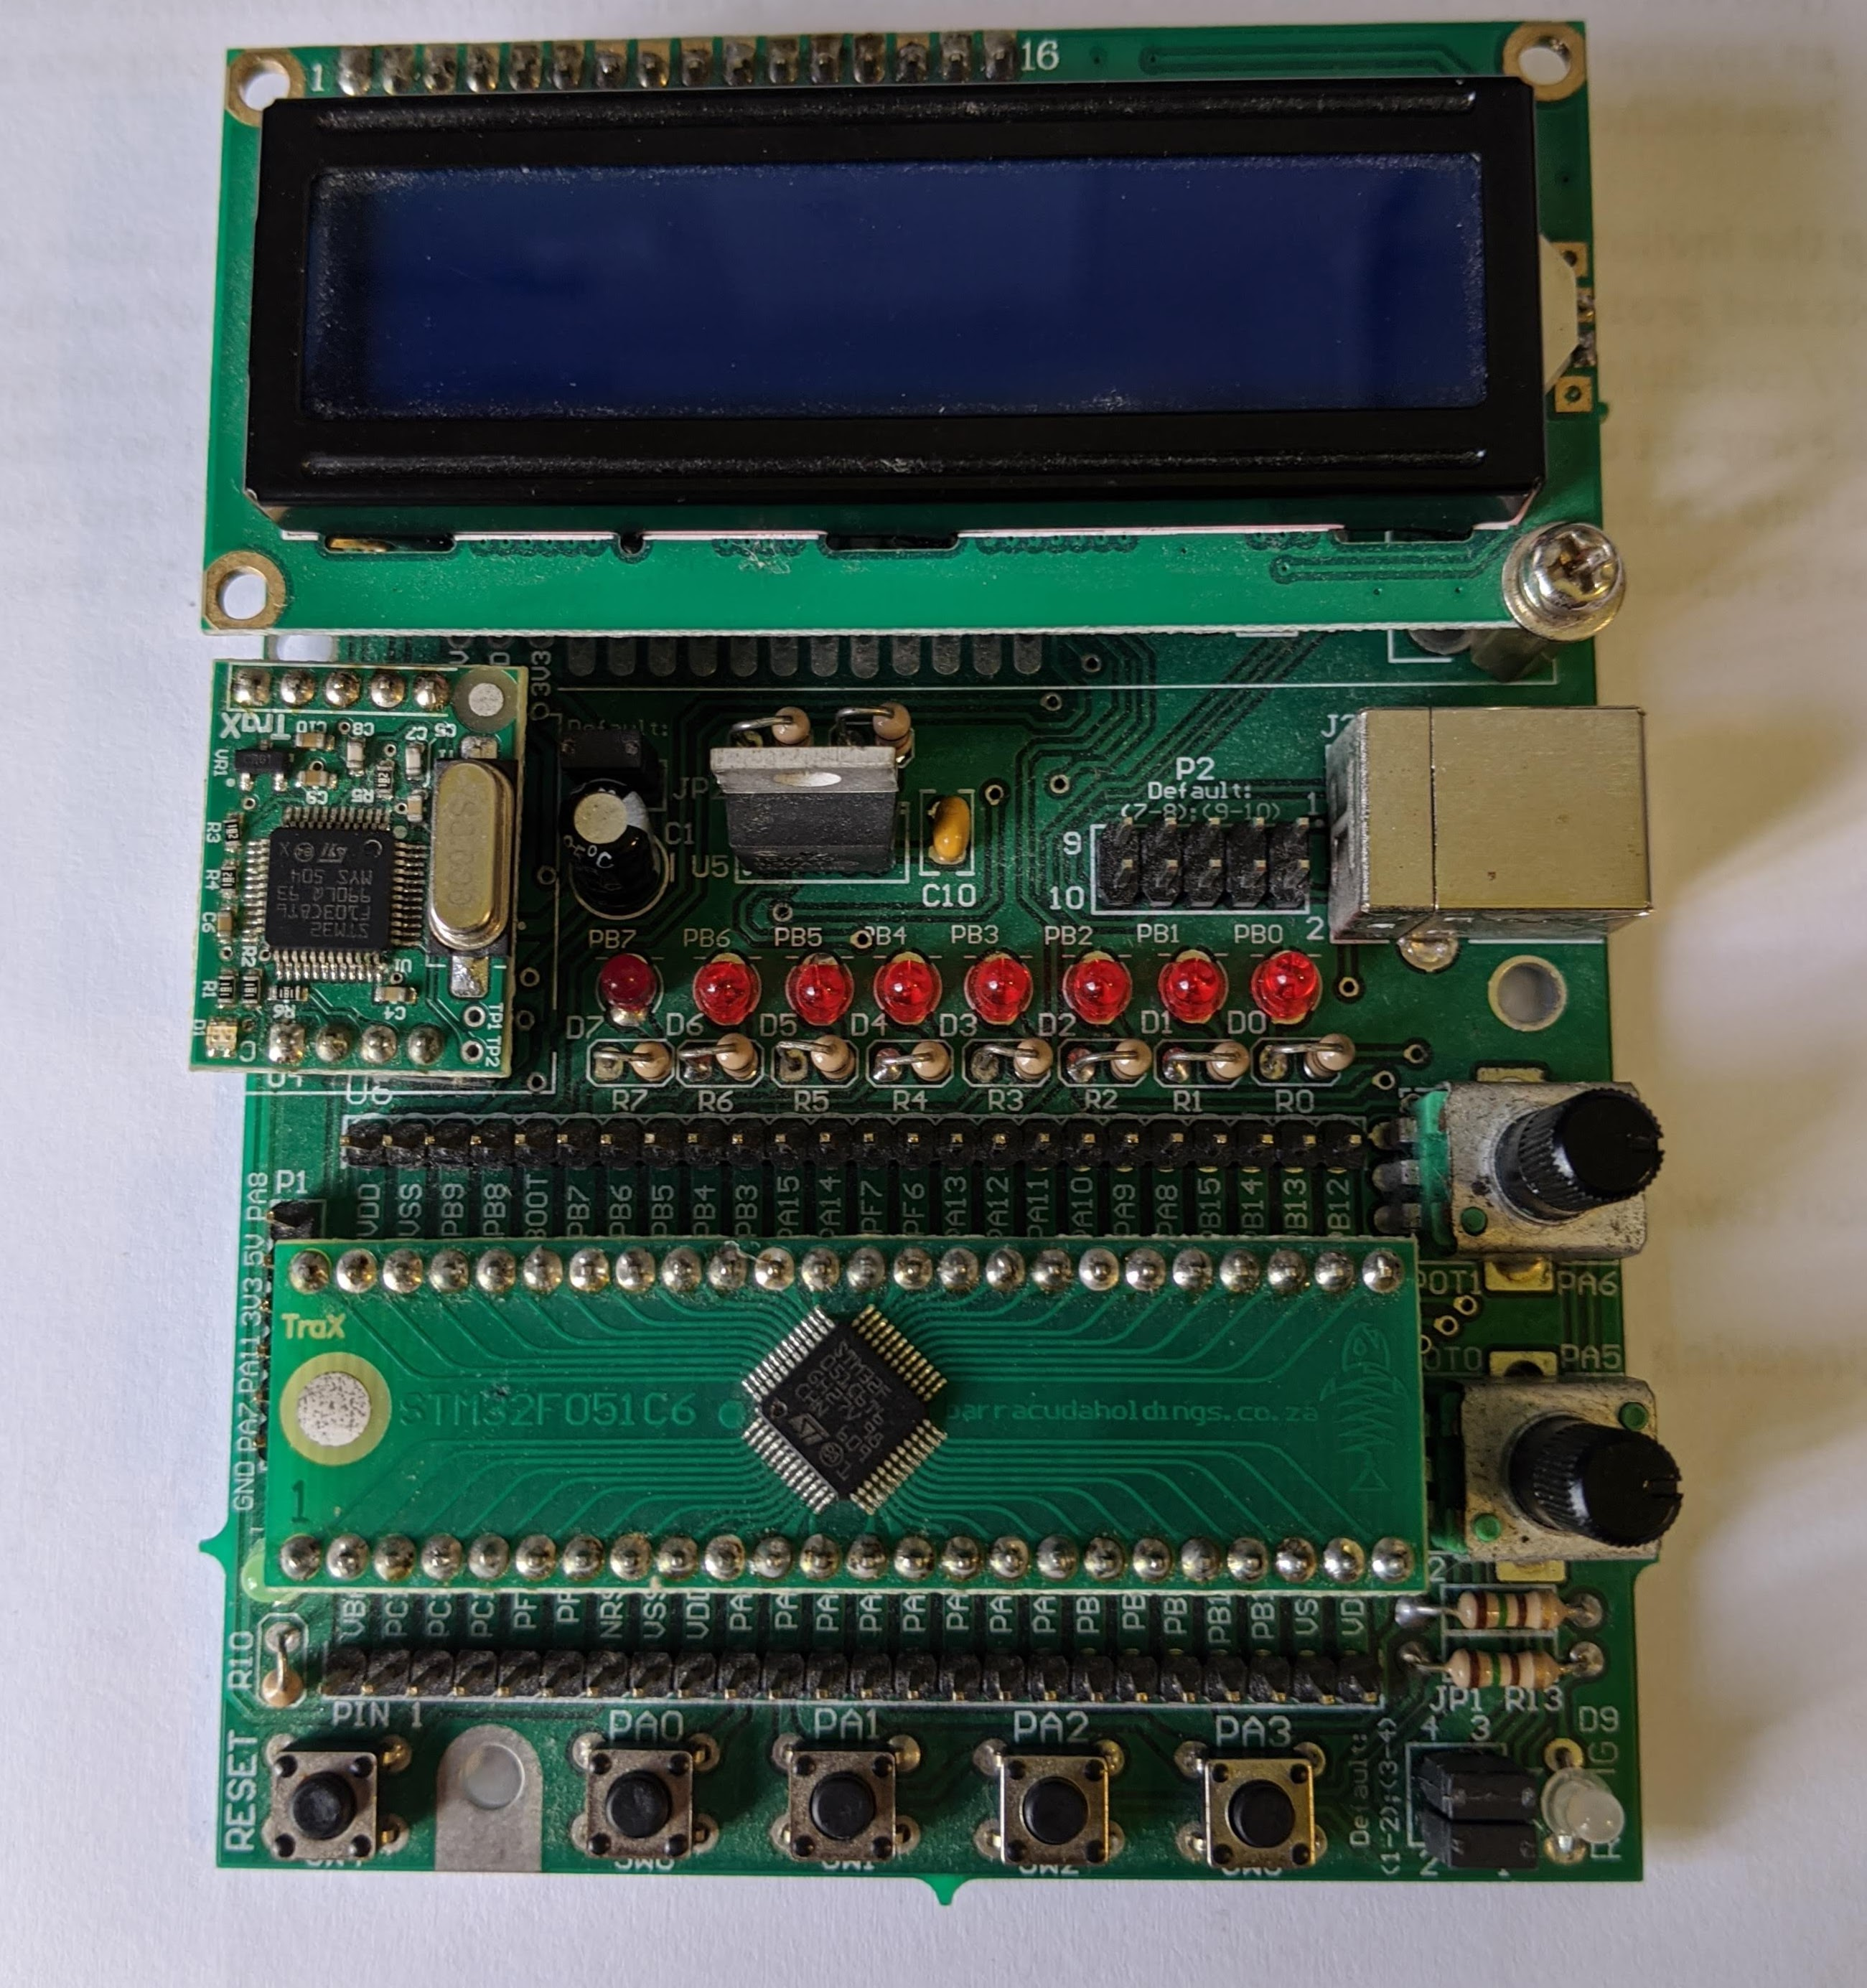
\includegraphics[width=.5\textwidth]{figures/design/dev_board_image.jpg}
	\caption{UCT STM32 Development Board}
	\label{fig:stm32_dev_board}
\end{figure}

The development board provides break-out pins for the microcontroller, 4 input buttons, an array of 8 LEDs, an LCD display and a built-in st-link v2 for debugging and programming the processor.

The STM32F051C6 was chosen partly because of its integration into the UCT development board making it easily obtainable at a low price and because of the following features

\begin{itemize}
	\item Analog to digital converter (ADC) peripheral
	\item Direct memory access (DMA) peripheral
	\item Timer peripherals with multiple interrupt channels
	\item Nested vectored interrupt controller (NVIC)
\end{itemize}



%%%%%%%%%%%%%%%%%%%%%%%%%%%%%%%%%%%%%%%%%%%%%%%%%%%%%%%%%%%



\subsection{Carrier Frequency Generator}
%Missing
% - Calculations and chosen values
\subsubsection{Functional Design}
To generate the 36kHz carrier waveform the LM555 timer IC was used. The module is designed to receive a 3.3V control signal. When a high logic level is received, the module switches the output at 36kHz to produce a square waveform.

The LED driver modules designed to be controlled by an open-collector, therefore a transistor was used to convert the push-pull output of the 555 timer to an open-collector output.

The 555 timer operates on the 5V supply connected to the module, therefore transistors were used to convert the 3.3V control signal to a 5V input for the RST pin.

\subsubsection{Schematic}
Figure \ref{fig:schematic_carrier_generation} below shows the schematic for the module.

\begin{figure}[H]
	\centering
	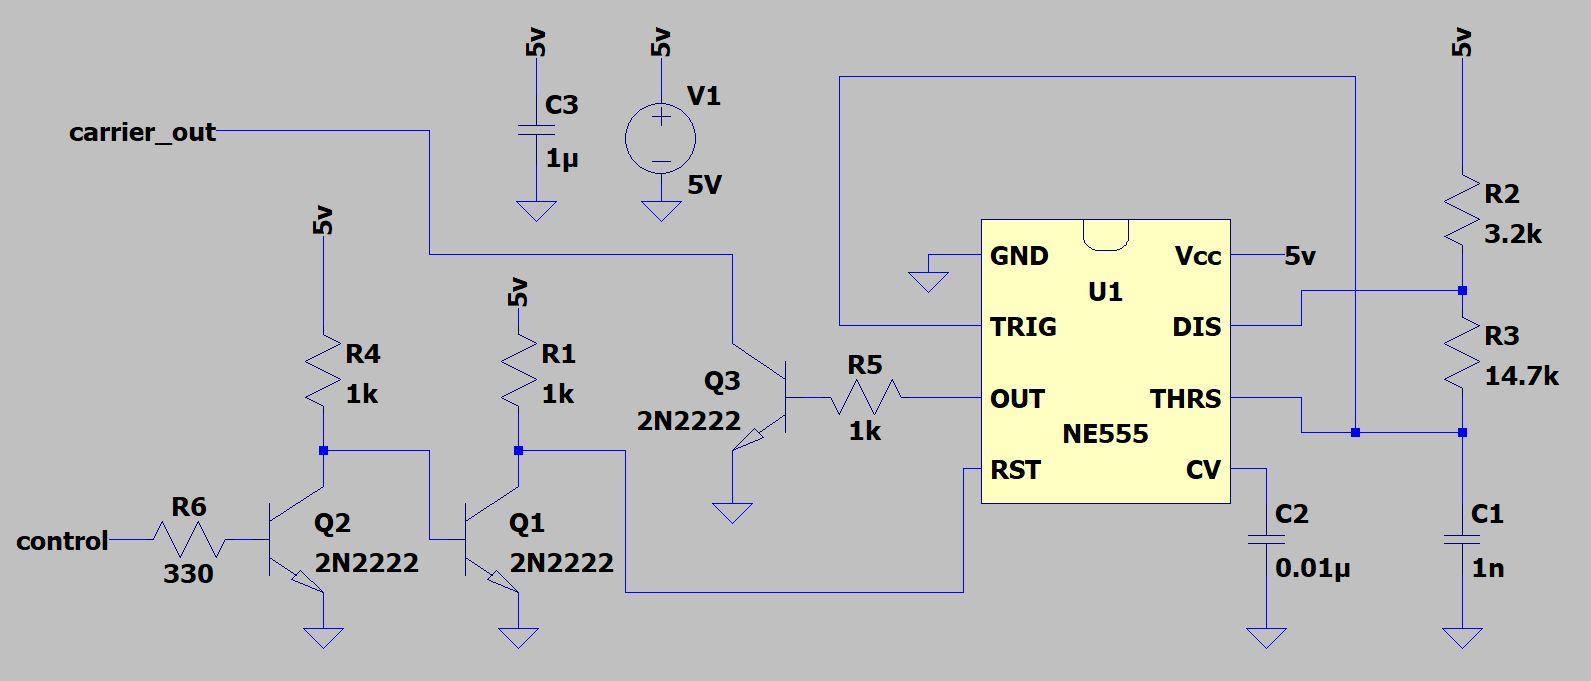
\includegraphics[width=.8\textwidth]{figures/design/carrier_waveform_generator_555.JPG}
	\caption{Carrier Generation Module Schematic}
	\label{fig:schematic_carrier_generation}
\end{figure}

\subsubsection{Frequency Generation}
%todo: this needs to be completed

According to the data sheet the period my be calculated as \(T = 0.693 (R_2 + 2R_3) C1\). A capacitor value of 10nF was chosen. Therefore, to generate a waveform with the desired period of $27.7\mu S$ the required theoretical value of $(R_2 + 2R_3)$ is $4k\Omega$.
%todo: finnish explaining resistor choice

%todo: finnish this paragraph
%After testing
The above design was implemented on a breadboard to test the

\subsubsection{Module Realization}
The strip-board implementation of the module is shown in figure \ref{fig:module_carrier_generation} below.

\begin{figure}[H]
	\centering
	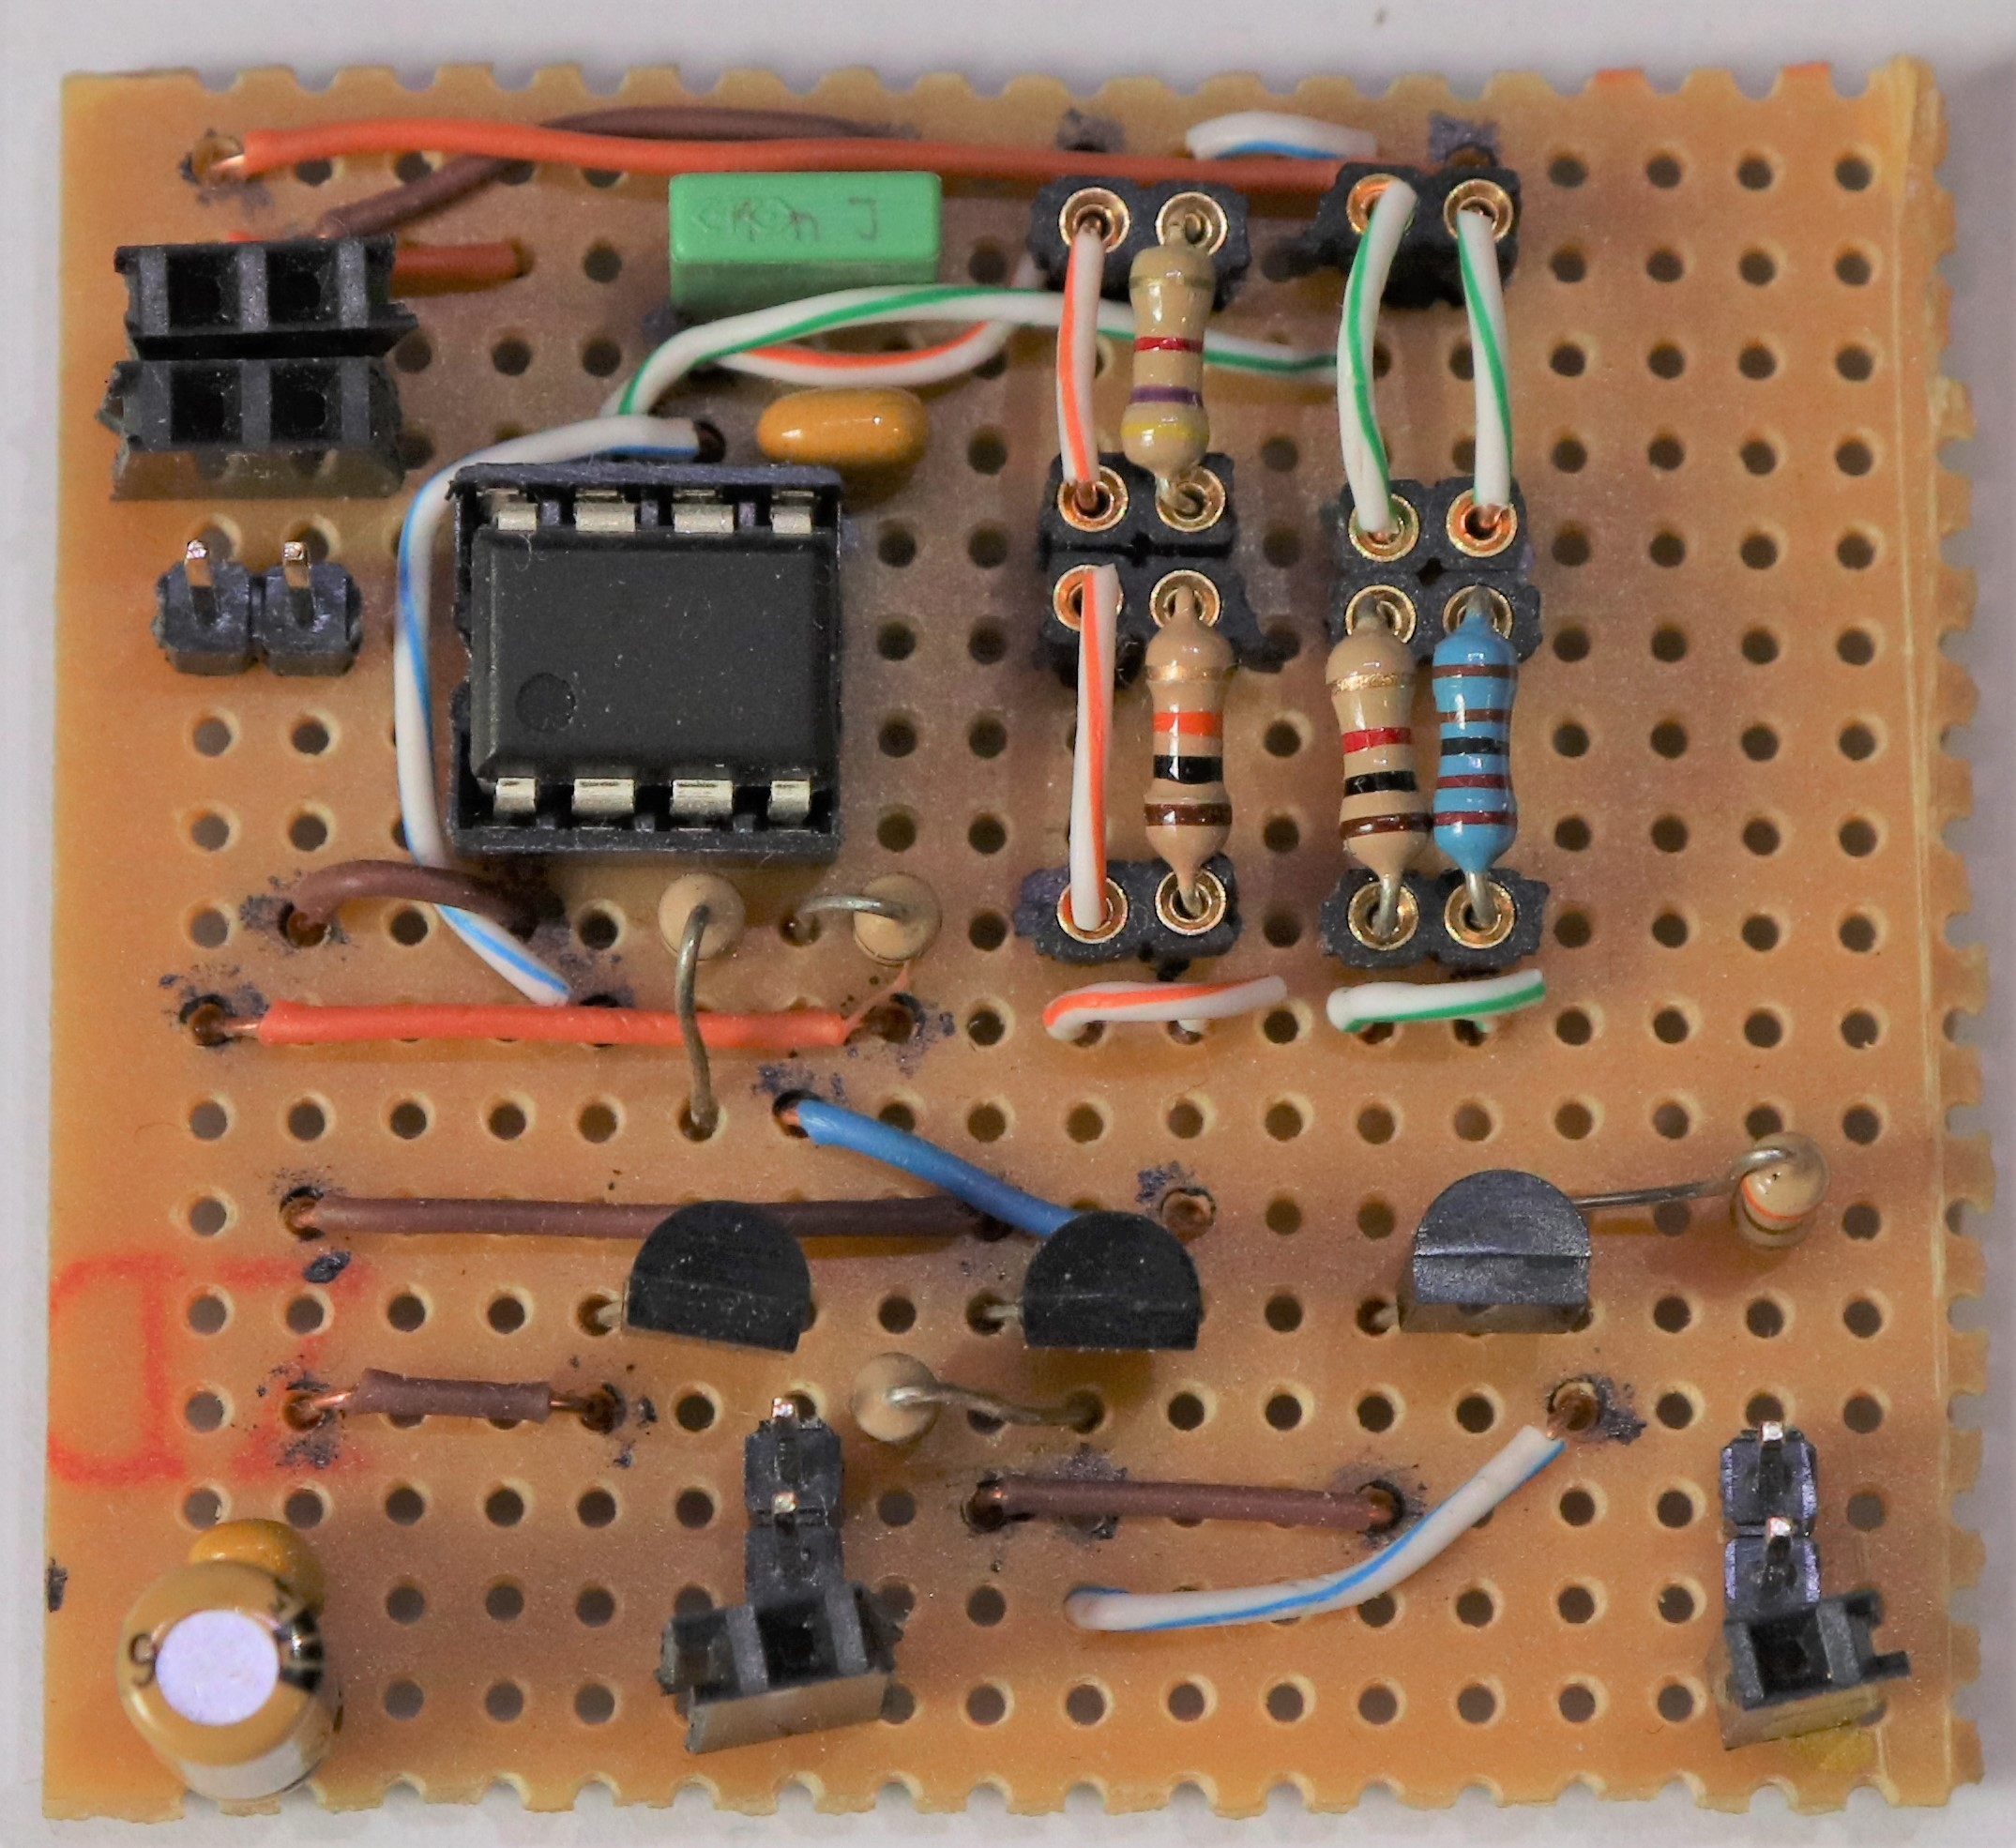
\includegraphics[width=.6\textwidth]{figures/modules/carrier_generator.jpg}
	\caption{Carrier Generation Module}
	\label{fig:module_carrier_generation}
\end{figure}



%%%%%%%%%%%%%%%%%%%%%%%%%%%%%%%%%%%%%%%%%%%%%%%%%%%%%%%%%%%



\subsection{Power LED Driver}

\subsubsection{Functional Design}
To operate the 3W high power IR LED a constant current driver module needed to be implemented. The module is designed to be controlled by an open-collector control signal such that when the control signal is pulled low the led is illuminated. The output of this module is a constant current designed to drive a power LED.

\subsubsection{Schematic}
Figure \ref{fig:schematic_power_led_driver} shows the design of a high power linear regulator, built around the IRLZ44 enhancement PMOSFET. Heat-sinks where attached to both the high power LED and the IRLZ44 power MOSFET.

\begin{figure}[H]
	\centering
	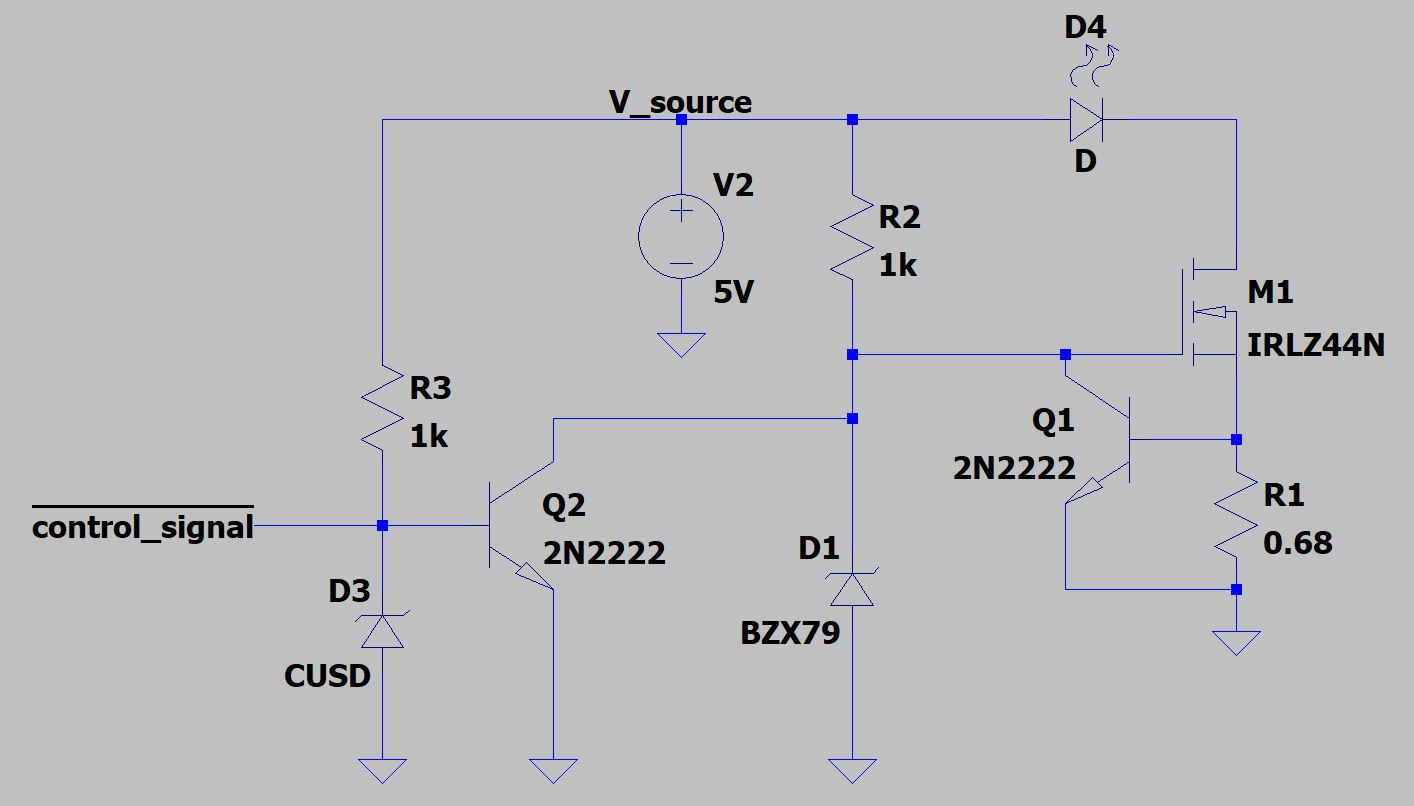
\includegraphics[width=.8\textwidth]{figures/design/power_led_driver.JPG}
	\caption{Power LED Driver Module Schematic}
	\label{fig:schematic_power_led_driver}
\end{figure}

\subsubsection{Constant Current Control}
%todo: Specs and component choice etc.

Because the LED needs to be modulated at 36kHz, standard LED driver ICs that use a switching regulator are not viable. This is because the switching frequency used in commonly available constant current switching regulators is not high enough. Instead a linear regulator was designed using discrete components.

%todo: explain how the circuit works


\subsubsection{Module Realization}
The strip-board implementation of the module is shown in figure \ref{fig:module_power_led_driver} below.

\begin{figure}[H]
	\centering
	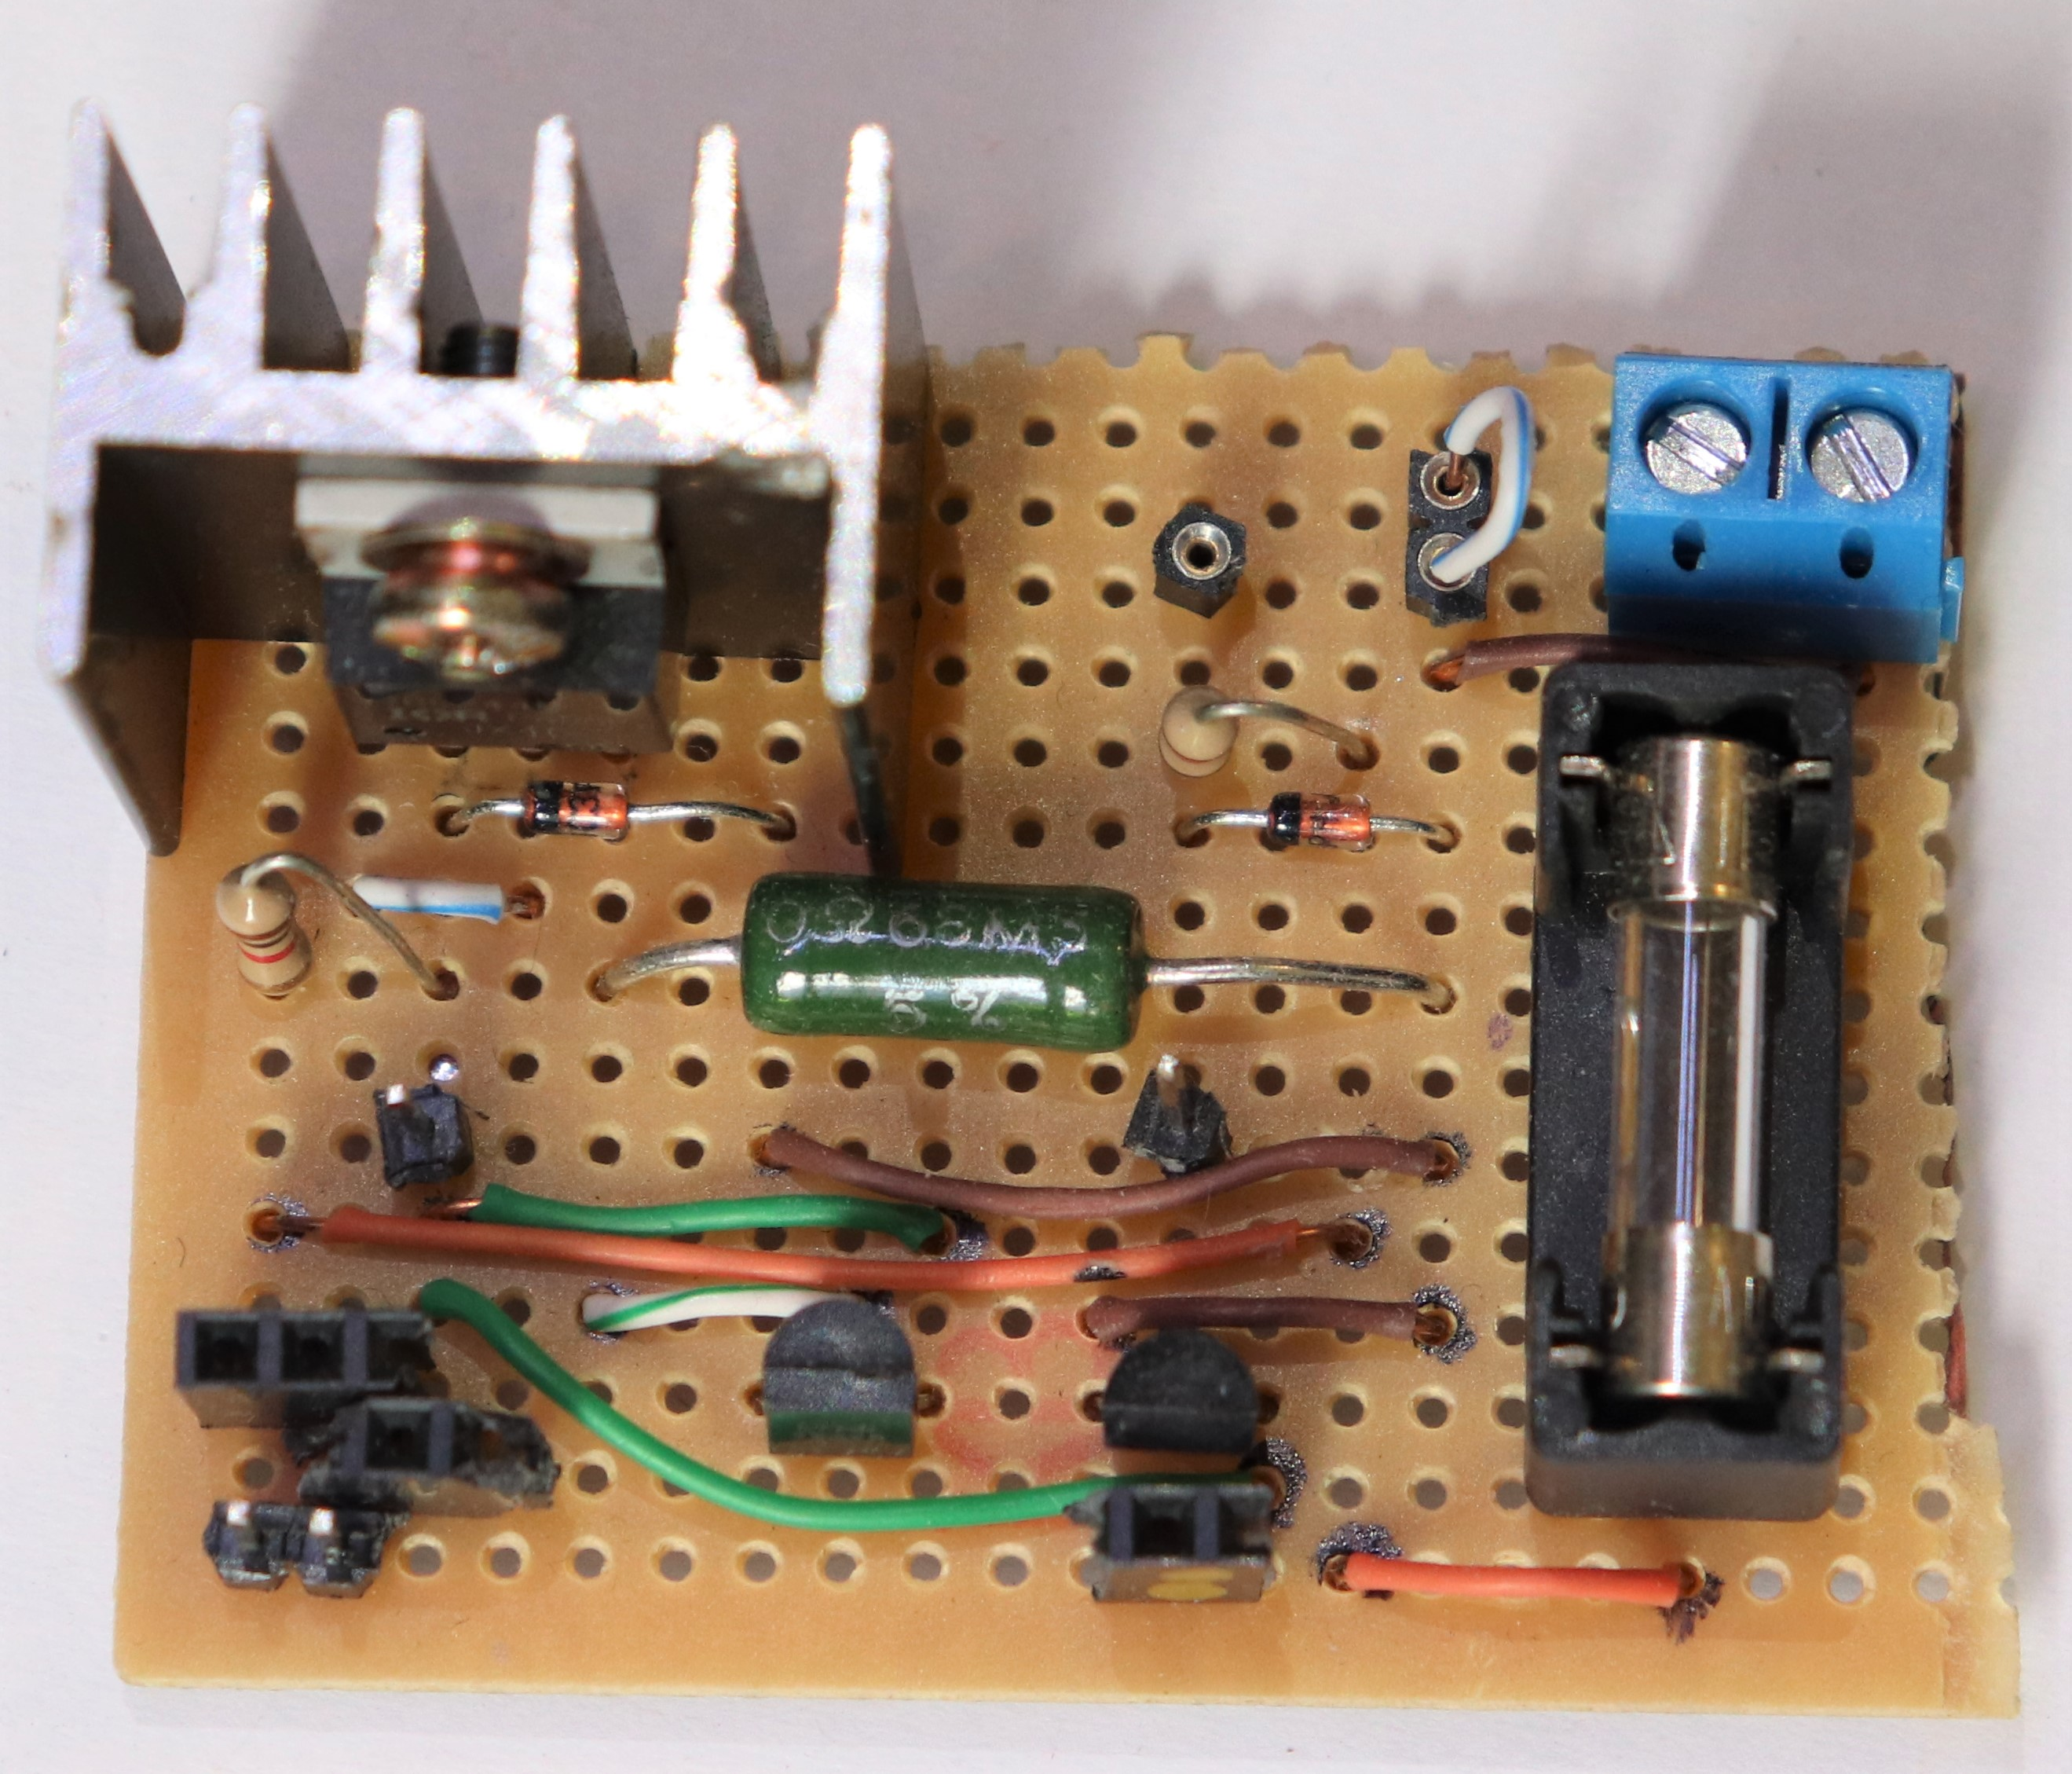
\includegraphics[width=.6\textwidth]{figures/modules/power_led_driver.jpg}
	\caption{Power LED Driver Module}
	\label{fig:module_power_led_driver}
\end{figure}



%%%%%%%%%%%%%%%%%%%%%%%%%%%%%%%%%%%%%%%%%%%%%%%%%%%%%%%%%%%




\subsection{LED Driver}

\subsubsection{Functional Design}
Due to the high power demands of the 3W IR LED, it is more appropriate to perform test and develop the communication protocol using a low power IR led. A separate low power LED driver module was designed for this specific purpose.

The module is designed to be pin-to-pin compatible with the power LED driver module, operating on the same input signal produced by an open-collector driven pin. Pulling the input low causes the LED to illuminate.



\subsubsection{Schematic}
Figure \ref{fig:schematic_low_power_led_driver} shows the schematic for this driver module.

\begin{figure}[H]
	\centering
	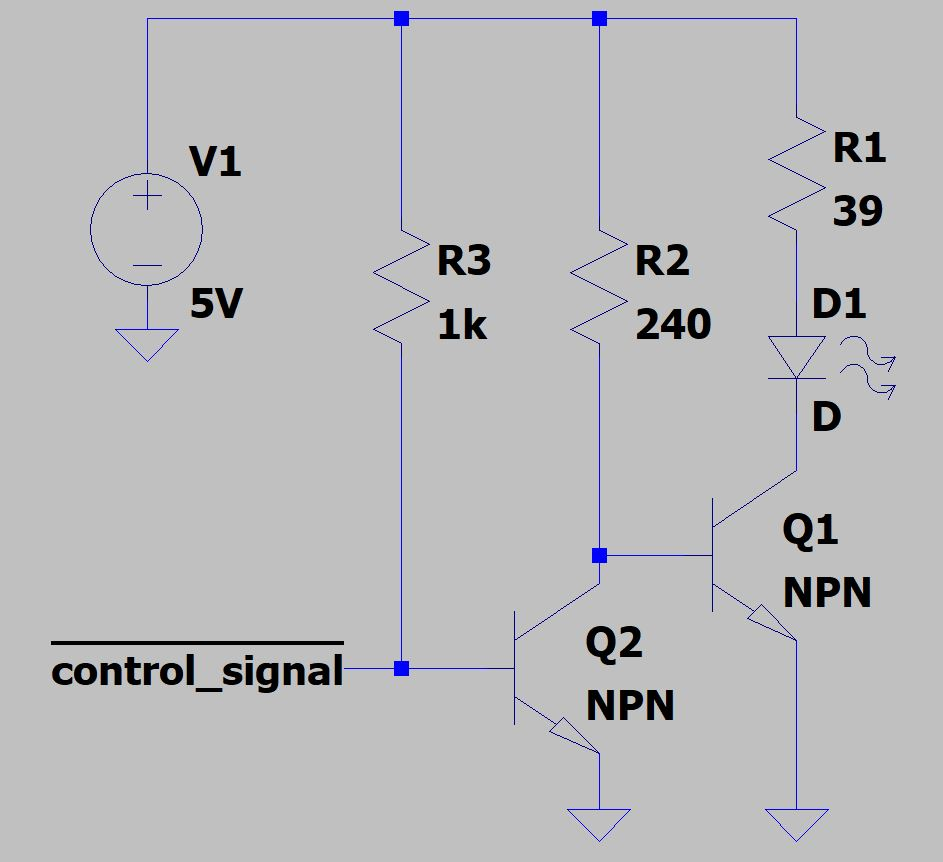
\includegraphics[width=.6\textwidth]{figures/design/low_power_led_driver.JPG}
	\caption{Low-Power LED Driver Module Schematic}
	\label{fig:schematic_low_power_led_driver}
\end{figure}

\subsubsection{Constant Current Control}
%todo: explain how constant current is created



\subsubsection{Module Realization}
The strip-board implementation of the module is shown in figure \ref{fig:module_led_driver} below.

\begin{figure}[H]
	\centering
	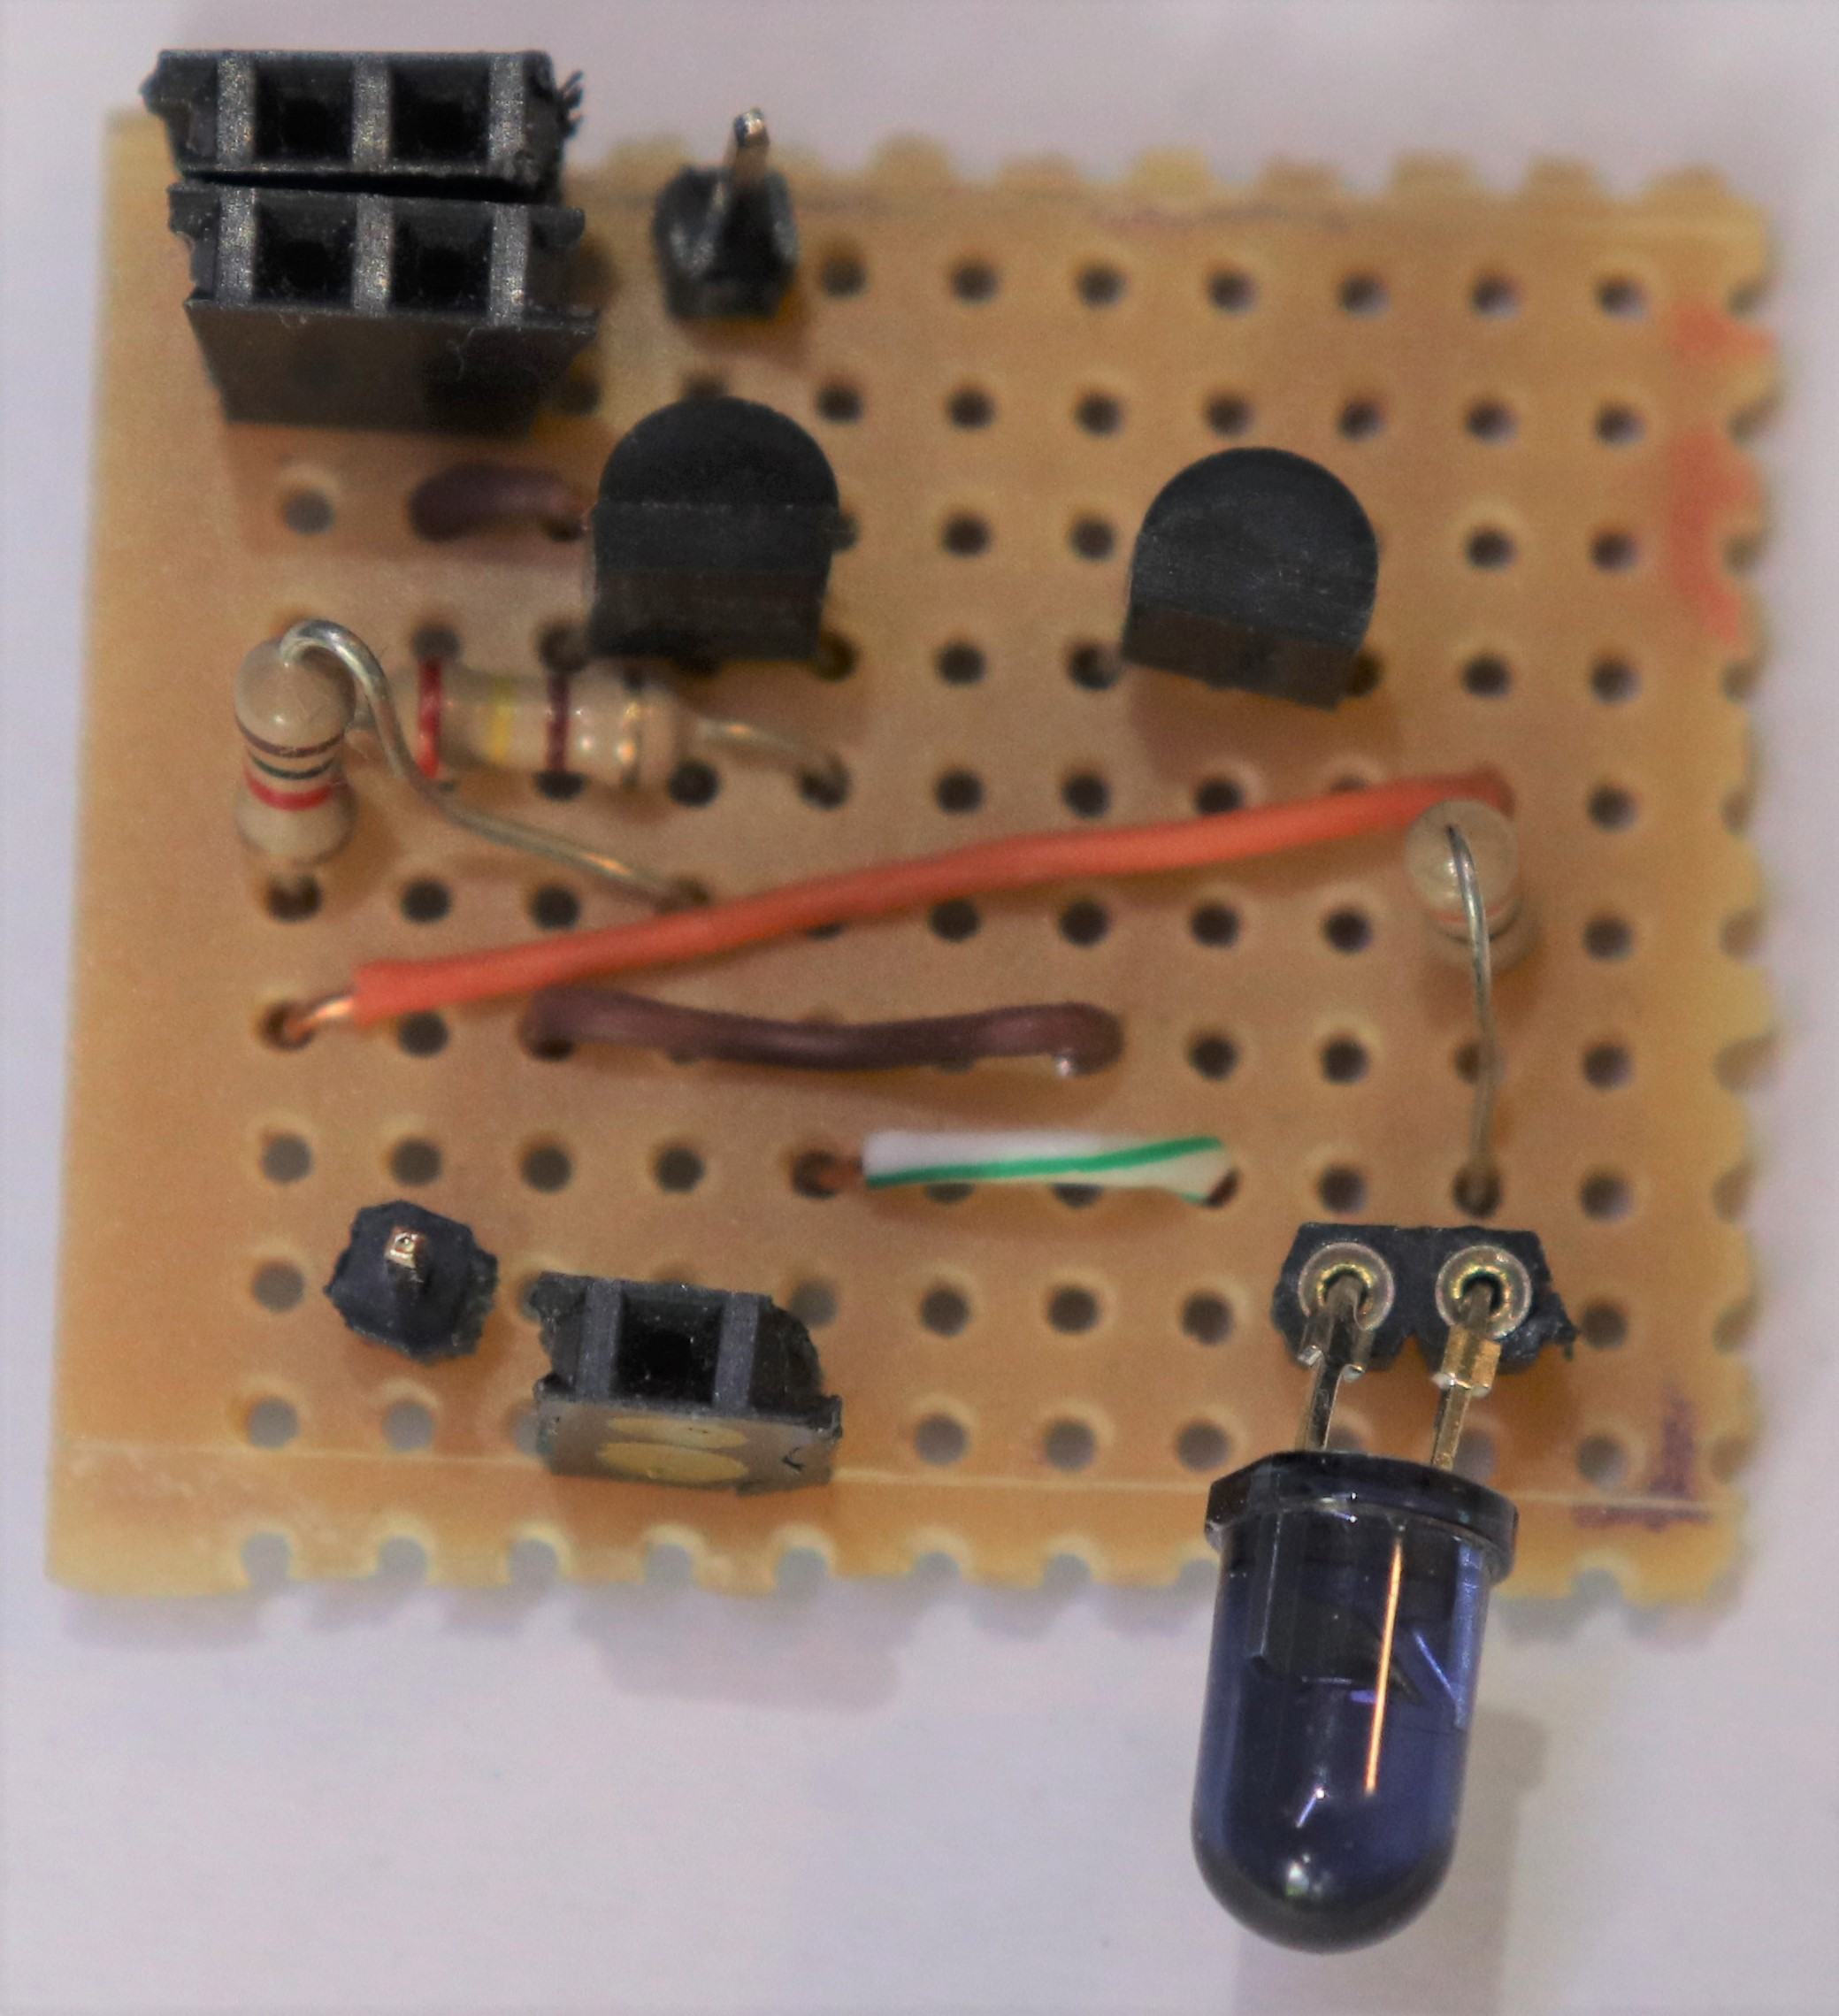
\includegraphics[width=.6\textwidth]{figures/modules/led_driver.jpg}
	\caption{LED Driver Module}
	\label{fig:module_led_driver}
\end{figure}




%%%%%%%%%%%%%%%%%%%%%%%%%%%%%%%%%%%%%%%%%%%%%%%%%%%%%%%%%%%




\subsection{Power LED Focus System}

\subsubsection{Functional Design}
The high power IR LED has a nominally wide beam angle. The function of the LED focus system is to efficiently generate a narrow beam of IR from this light source. This was achieved by using a lens to focus the light into a parallel beam and using a tube to prevent the light not passing through the lens from spilling into the surrounding environment.


\subsubsection{Construction}
Figure \ref{fig:light_focusing_tube} below shows an exploded view of this hardware module. The diagram lists the components used to construct the light focusing tube.

\begin{figure}[H]
	\centering
	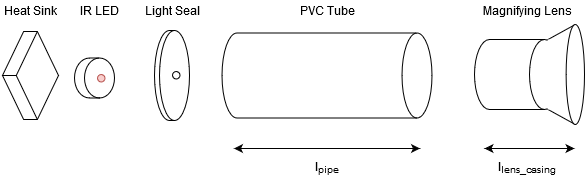
\includegraphics[width=.8\textwidth]{figures/design/beam_tube.png}
	\caption{Exploded View - Light Focusing Tube}
	\label{fig:light_focusing_tube}
\end{figure}

\paragraph{Component Dimensions}
The magnifying lens casing had a length of 30mm, the lens is in-set by 1mm and 3mm of the casing remains external to the tube. The experimental result from section \ref{exp:focal_length} calculated the focal length to be 53mm.

\subsubsection{Light Focusing}

A narrow beam of parallel rays of light may be formed using a point source and ideal lens. Approximating the LED as a point source and the magnifying lens as ideal, a narrow beam may be generated by positioning the light source one focal length away from the lens.

The distance between the light source and lens can be calculated according to equation \ref{eqn:tube_length}.

\begin{equation}
	d_{source-lens} = l_{tube} - l_{lens\_casing} + (l_{lens\_inset\_distance} + l_{lens\_external}) + l_{light\_seal\_thickness}
	\label{eqn:tube_length}
\end{equation}

$d_{source-lens}$ is the distance between the light source and the lens. $l_{tube}$ is the length of the tube. $l_{lens\_casing}$ is the length of the magnifying lens casing as illustrated in figure \ref{fig:light_focusing_tube}, $l_{lens\_inset\_distance}$ is the amount by which the lens is in-set inside the casing and $l_{lens\_external}$ is a measure of the length of casing that remains external to the tube. $l_{light\_seal\_thickness}$ is a measure of the thickness of the hard-board used to form the light seal.

The length $l_{tube}$ was calculated by substituting the experimentally determined focal length into the equation as the length $d_{source-lens}$.

Substituting these values into equation \ref{eqn:tube_length}, the length $l_{tube}$ was calculated

\[l_{tube} = d_{source-lens} + l_{lens\_casing} - (l_{lens\_inset\_distance} + l_{lens\_external}) - l_{light\_seal\_thickness}\]

\[l_{tube} = 53mm + 30mm - (1mm + 3mm) - 3mm = 76mm\]


\subsubsection{Module Realization}
The implementation of the light focus system is shown in figure \ref{fig:module_light_focus} below. Excluded from this image is the IR led and heat-sink.

\begin{figure}[H]
	\centering
	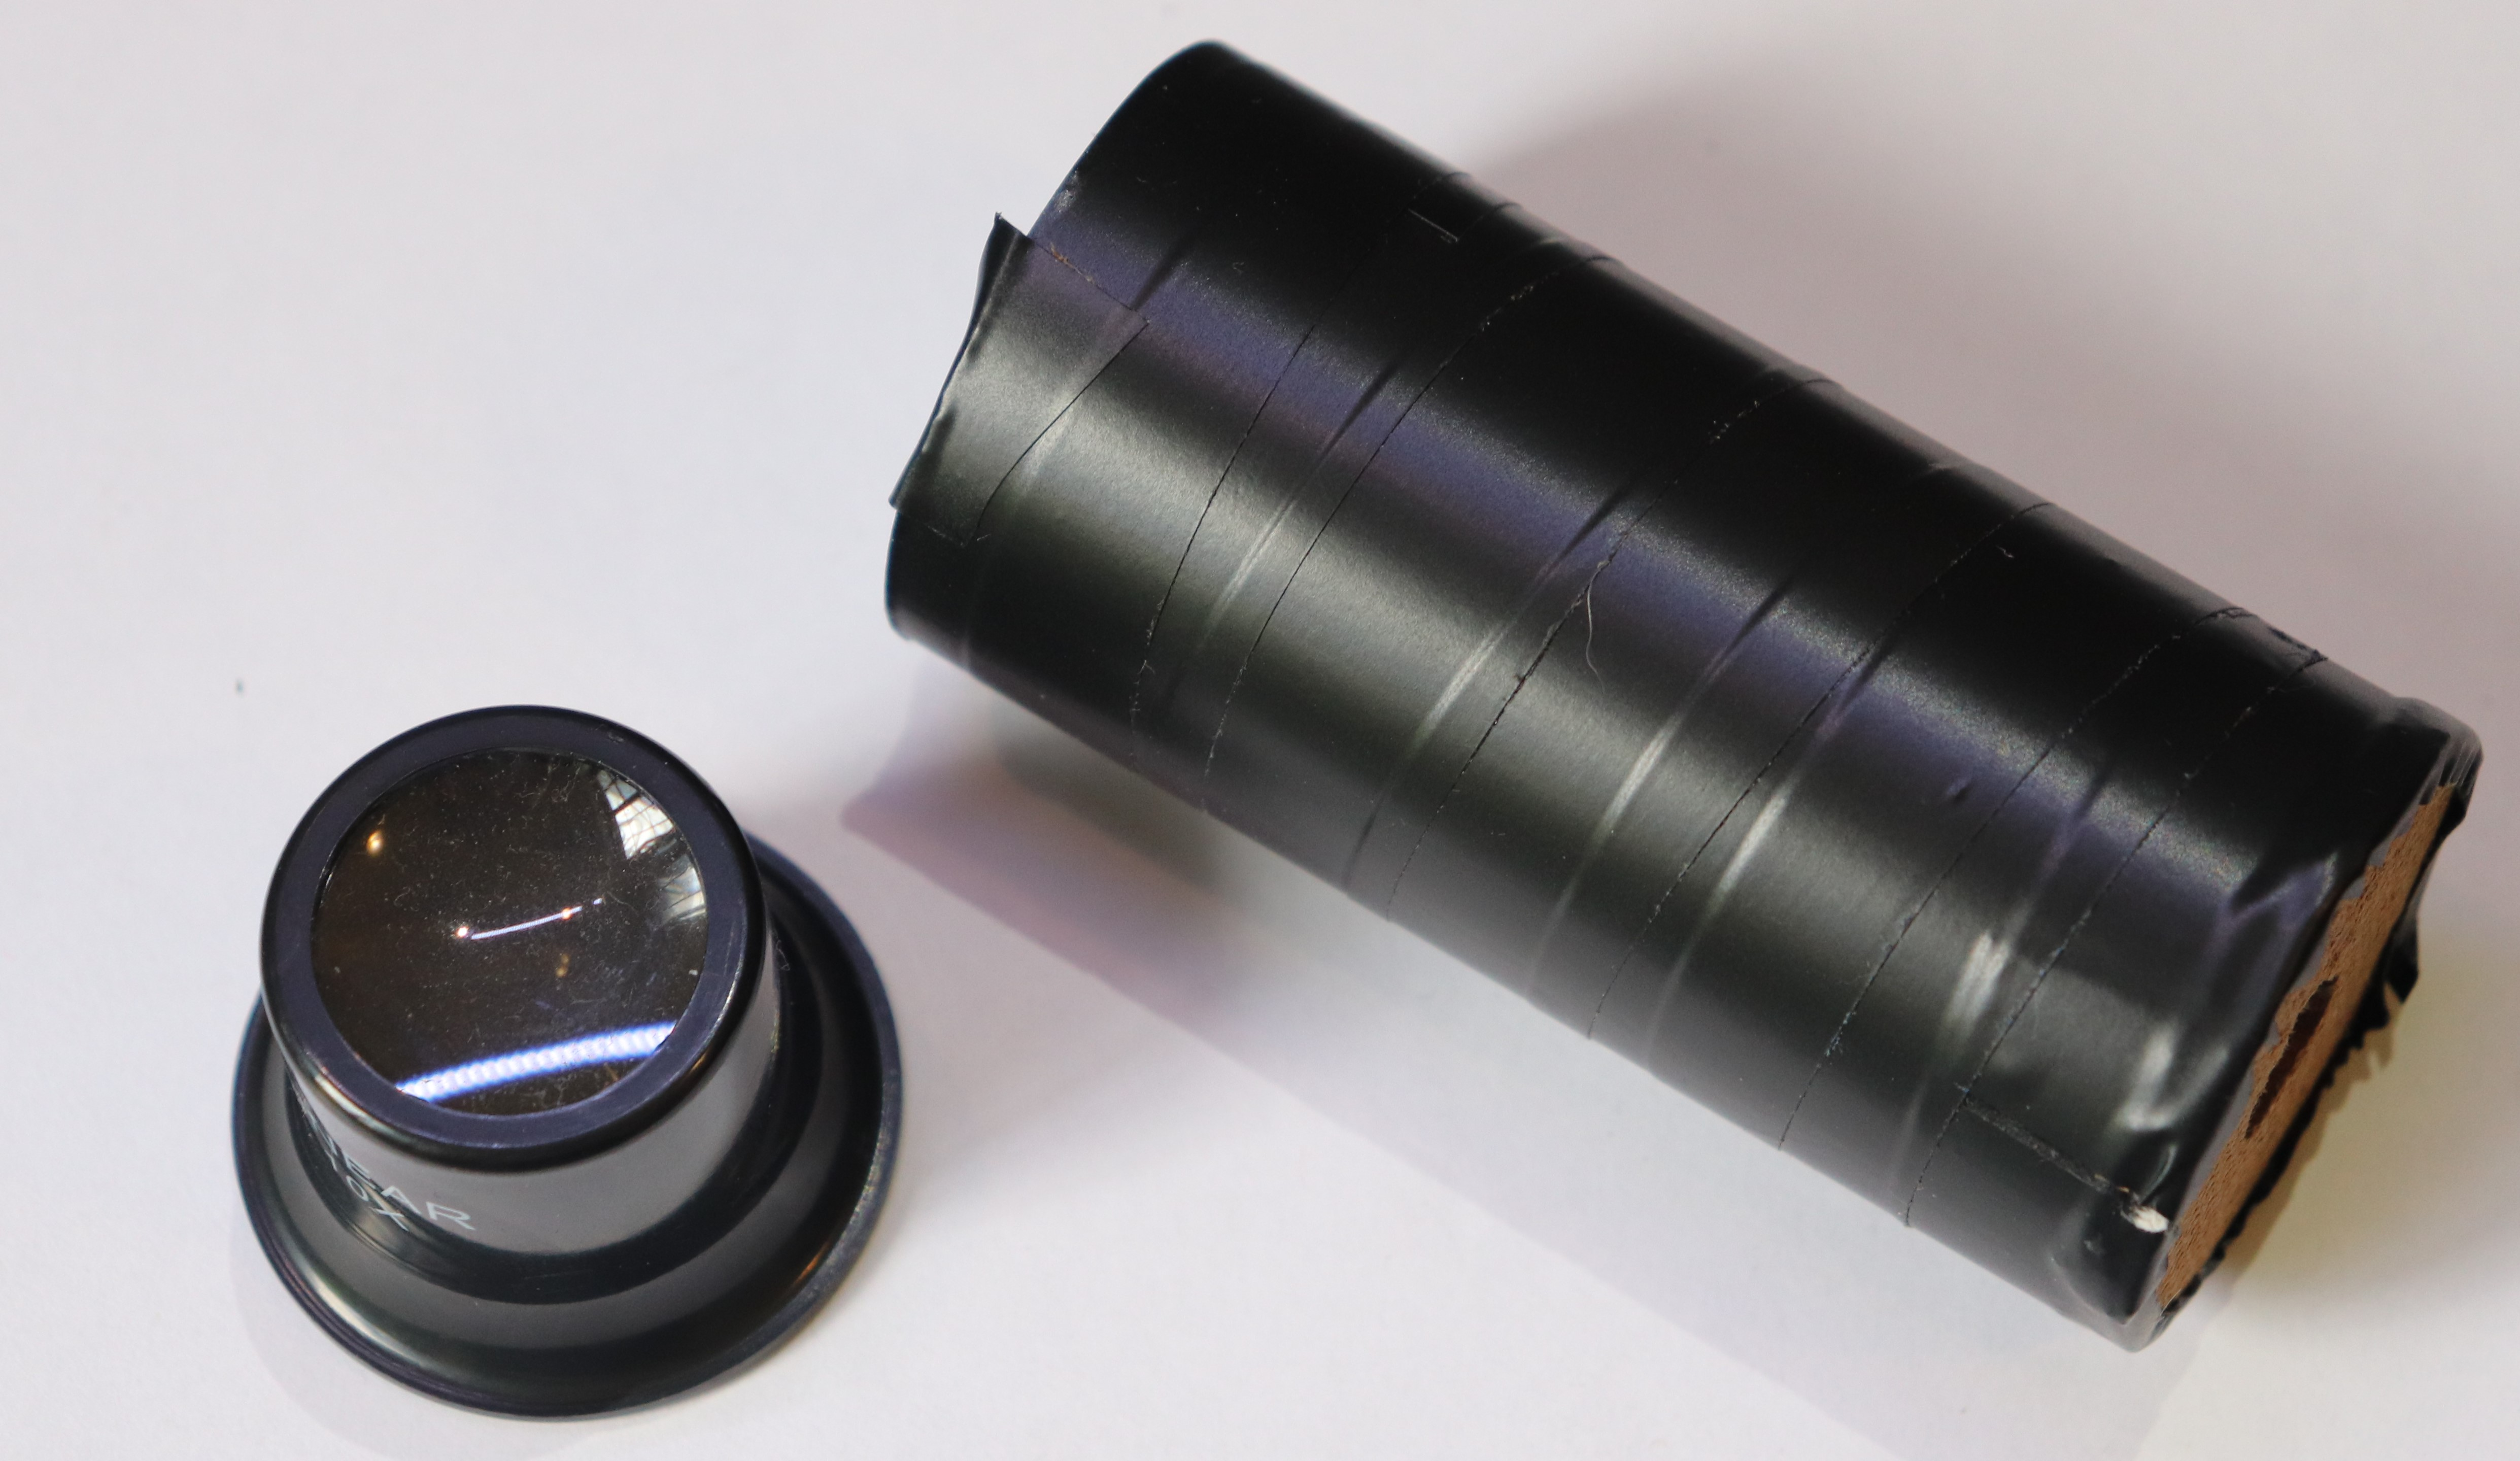
\includegraphics[width=.6\textwidth]{figures/modules/light_focus_tube_lens.jpg}
	\caption{Light Focus System}
	\label{fig:module_light_focus}
\end{figure}



%%%%%%%%%%%%%%%%%%%%%%%%%%%%%%%%%%%%%%%%%%%%%%%%%%%%%%%%%%%




\subsection{Photodiode IR Detector}
%Missing:
% - Schematic and explaination
% - Talk about MCP6022 and important specs

\subsubsection{Functional Design}
The photodiode IR detector module is designed to convert fluctuations in infrared radiation into a voltage signal. The circuit is designed to produce an output voltage proportional to changes in the current flowing through the photodiode.


\subsubsection{Schematic}
Figure \ref{fig:schematic_photodiode_transimpedance} below shows the schematic for the module. The circuit is inspired by S. Schrires 'Infrared Radio Link' circuit which is found in the EEE3071 course notes \cite{Schrire2007}.


\begin{figure}[H]
	\centering
	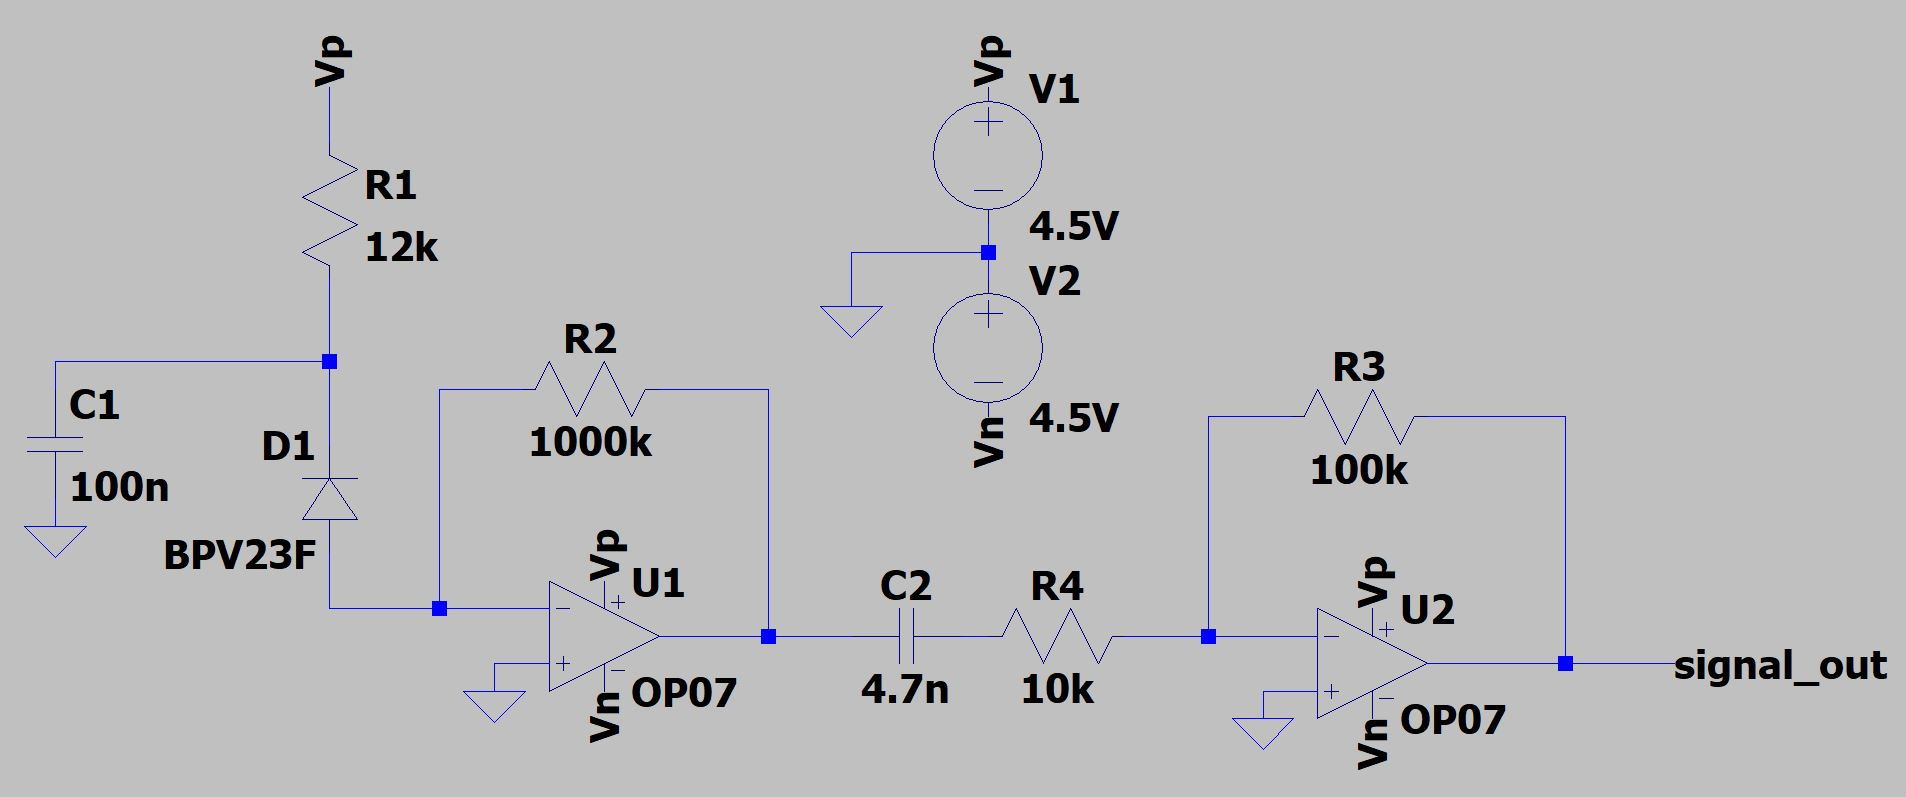
\includegraphics[width=.8\textwidth]{figures/design/photodiode_transimpedance.JPG}
	\caption{Photodiode IR Detector Module Schematic}
	\label{fig:schematic_photodiode_transimpedance}
\end{figure}

\subsubsection{Trans-impedance Amplifier}
%todo: this needs to be completed


\subsubsection{Module Realization}
The strip-board implementation of the module is shown in figure \ref{fig:module_photodiode_receiver} below.

\begin{figure}[H]
	\centering
	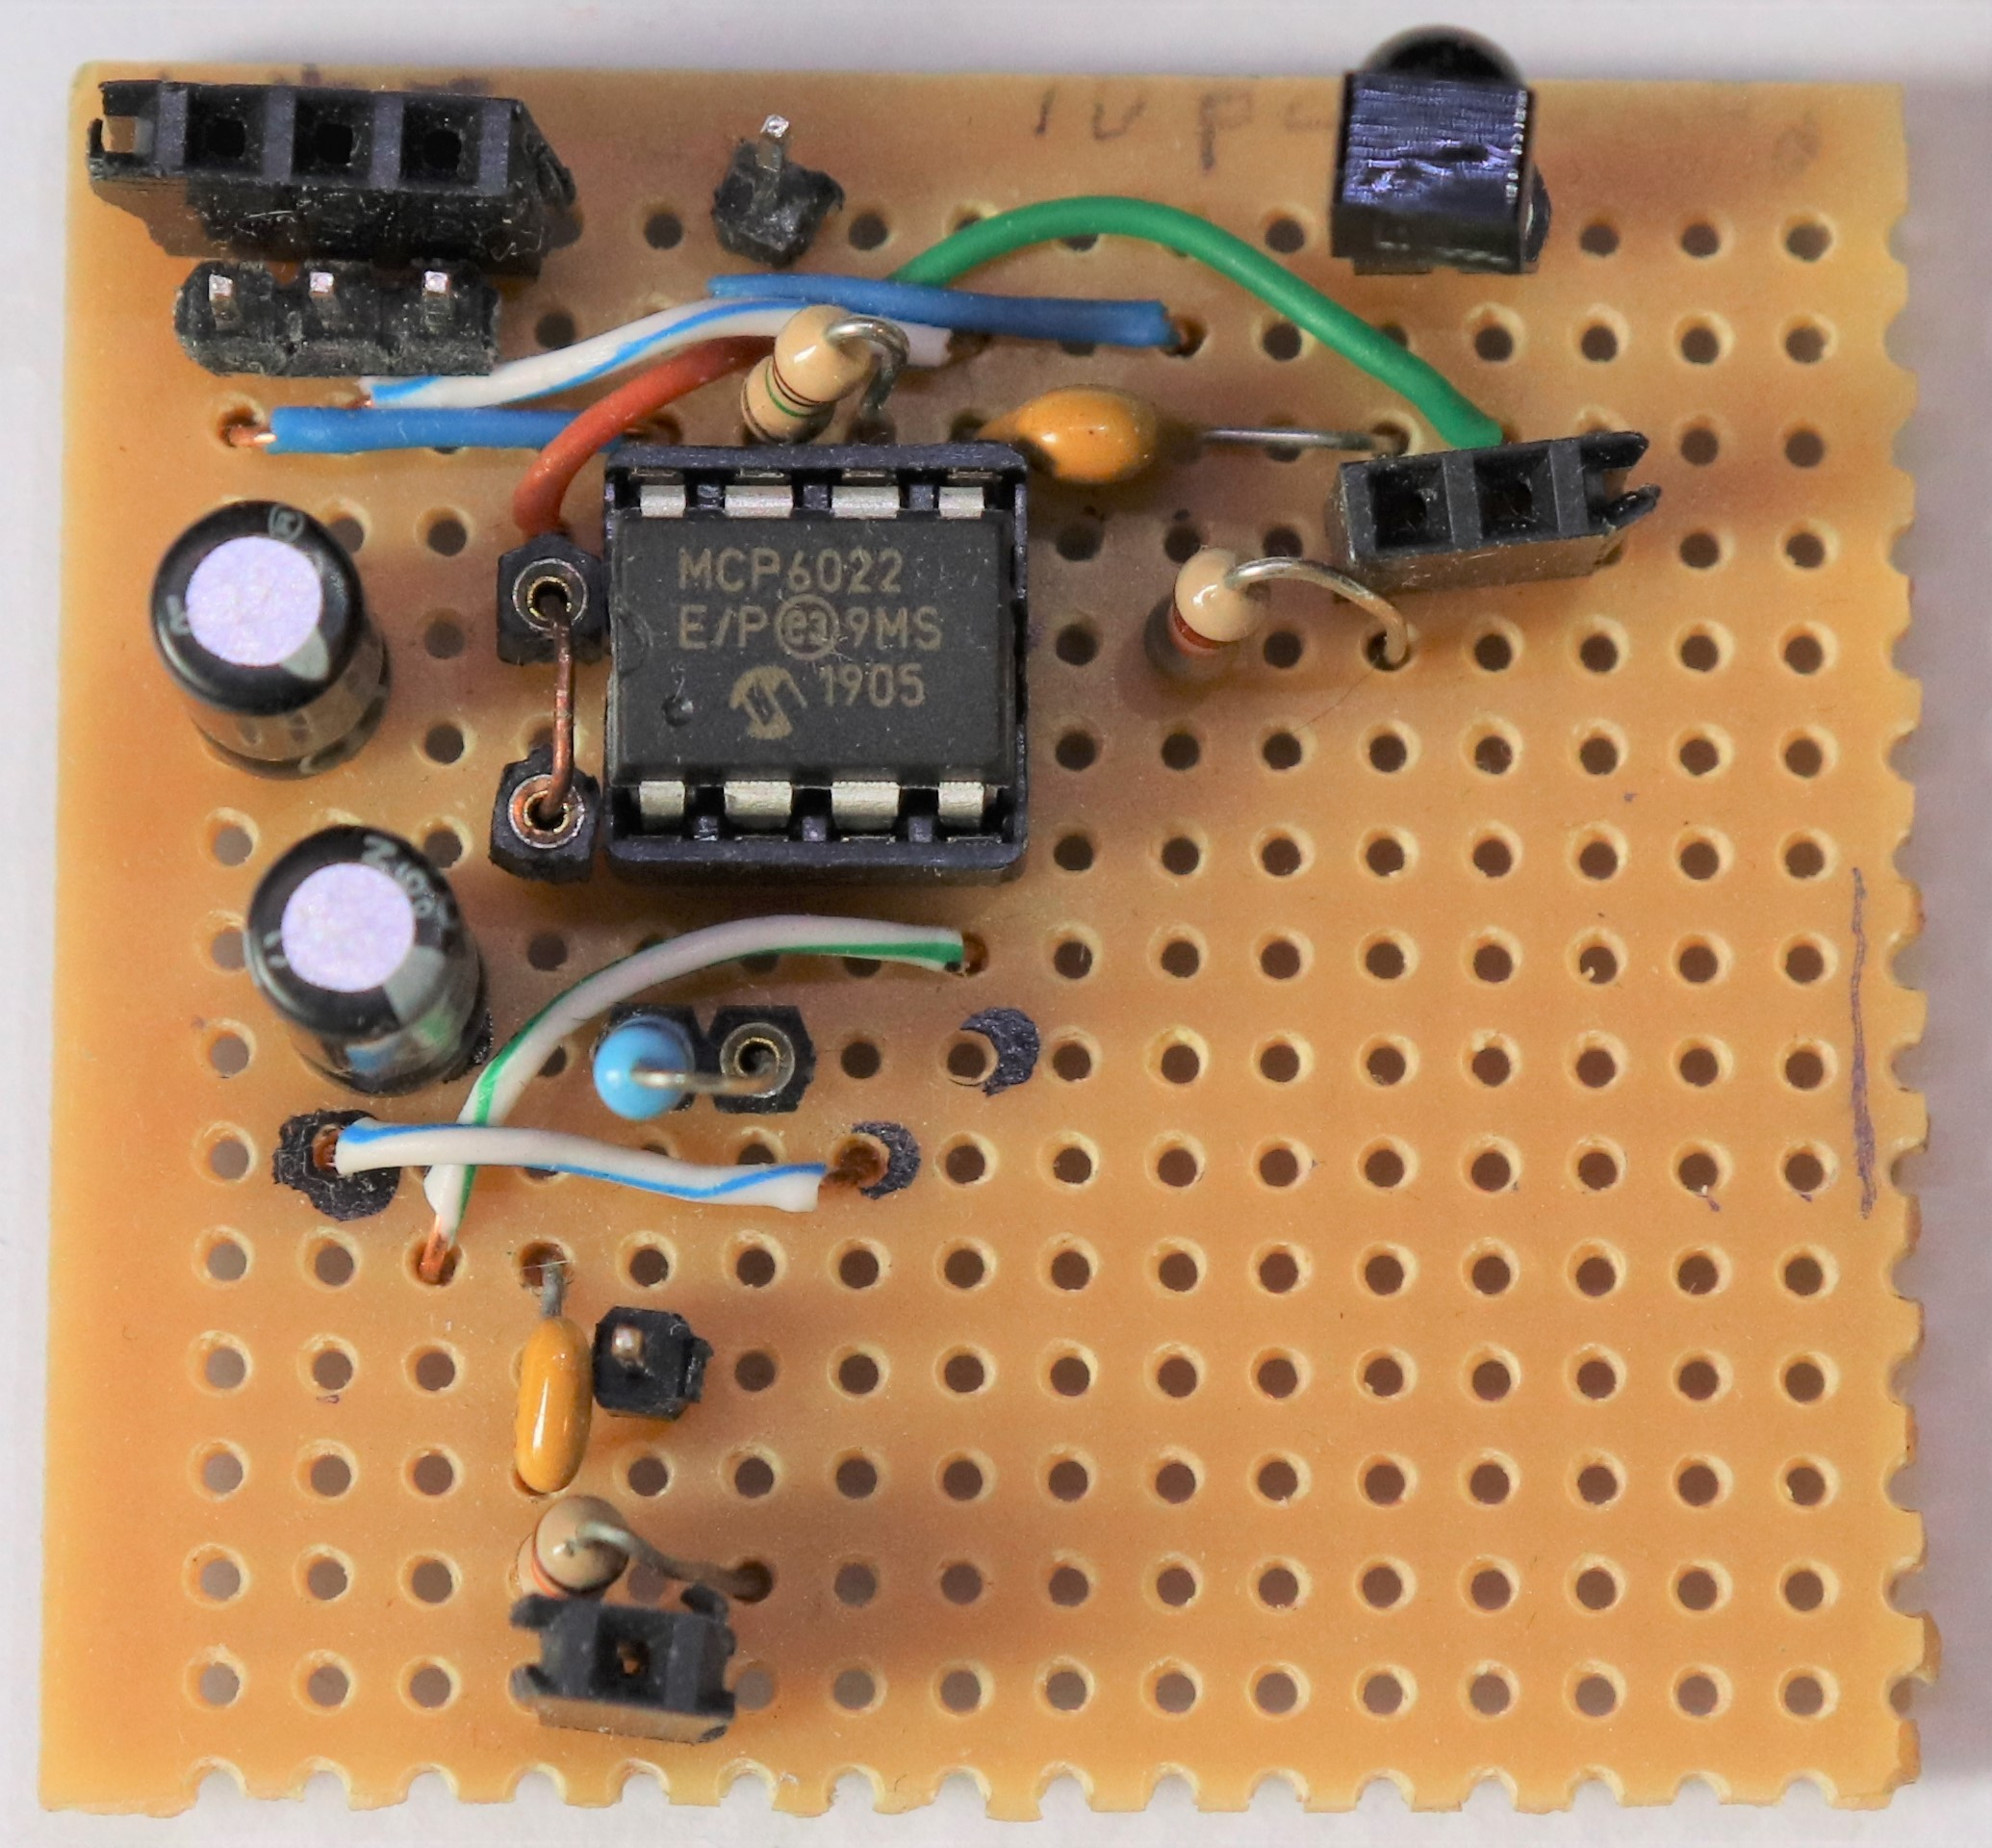
\includegraphics[width=.6\textwidth]{figures/modules/photodiode_receiver.jpg}
	\caption{Photodiode IR Receiver Module}
	\label{fig:module_photodiode_receiver}
\end{figure}


%%%%%%%%%%%%%%%%%%%%%%%%%%%%%%%%%%%%%%%%%%%%%%%%%%%%%%%%%%%



\subsection{Phototransistor IR Detector}

\subsubsection{Functional Design}
The phototransistor IR detector module, like the photodiode IR detector module, is designed to convert fluctuation in infrared radiation into a voltage signal. The circuit is designed to produce an output voltage proportional to changes in the current flowing through the phototransistor.

\subsubsection{Schematic}
Figure \ref{fig:schematic_phototransistor_detector} below shows the schematic for the module.


\begin{figure}[H]
	\centering
	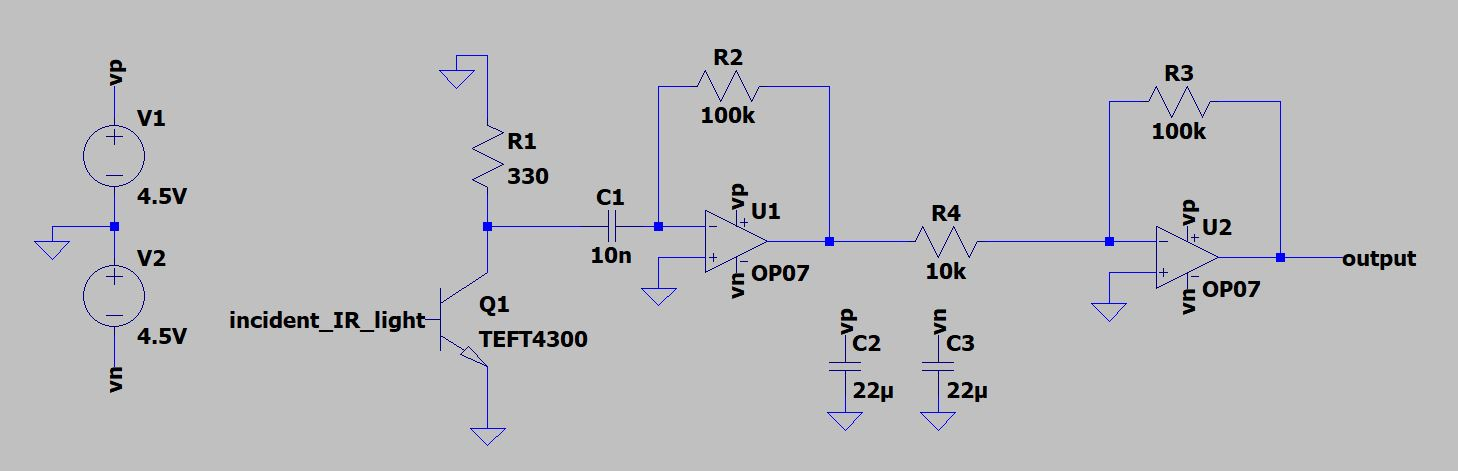
\includegraphics[width=.9\textwidth]{figures/design/phototransistor_detector.JPG}
	\caption{Phototransistor IR Detector Module Schematic}
	\label{fig:schematic_phototransistor_detector}
\end{figure}

\subsubsection{Trans-impedance Amplifier}
%todo: this needs to be completed


\subsubsection{Module Realization}
The strip-board implementation of the module is shown in figure \ref{fig:module_photodiode_receiver} below.

\begin{figure}[H]
	\centering
	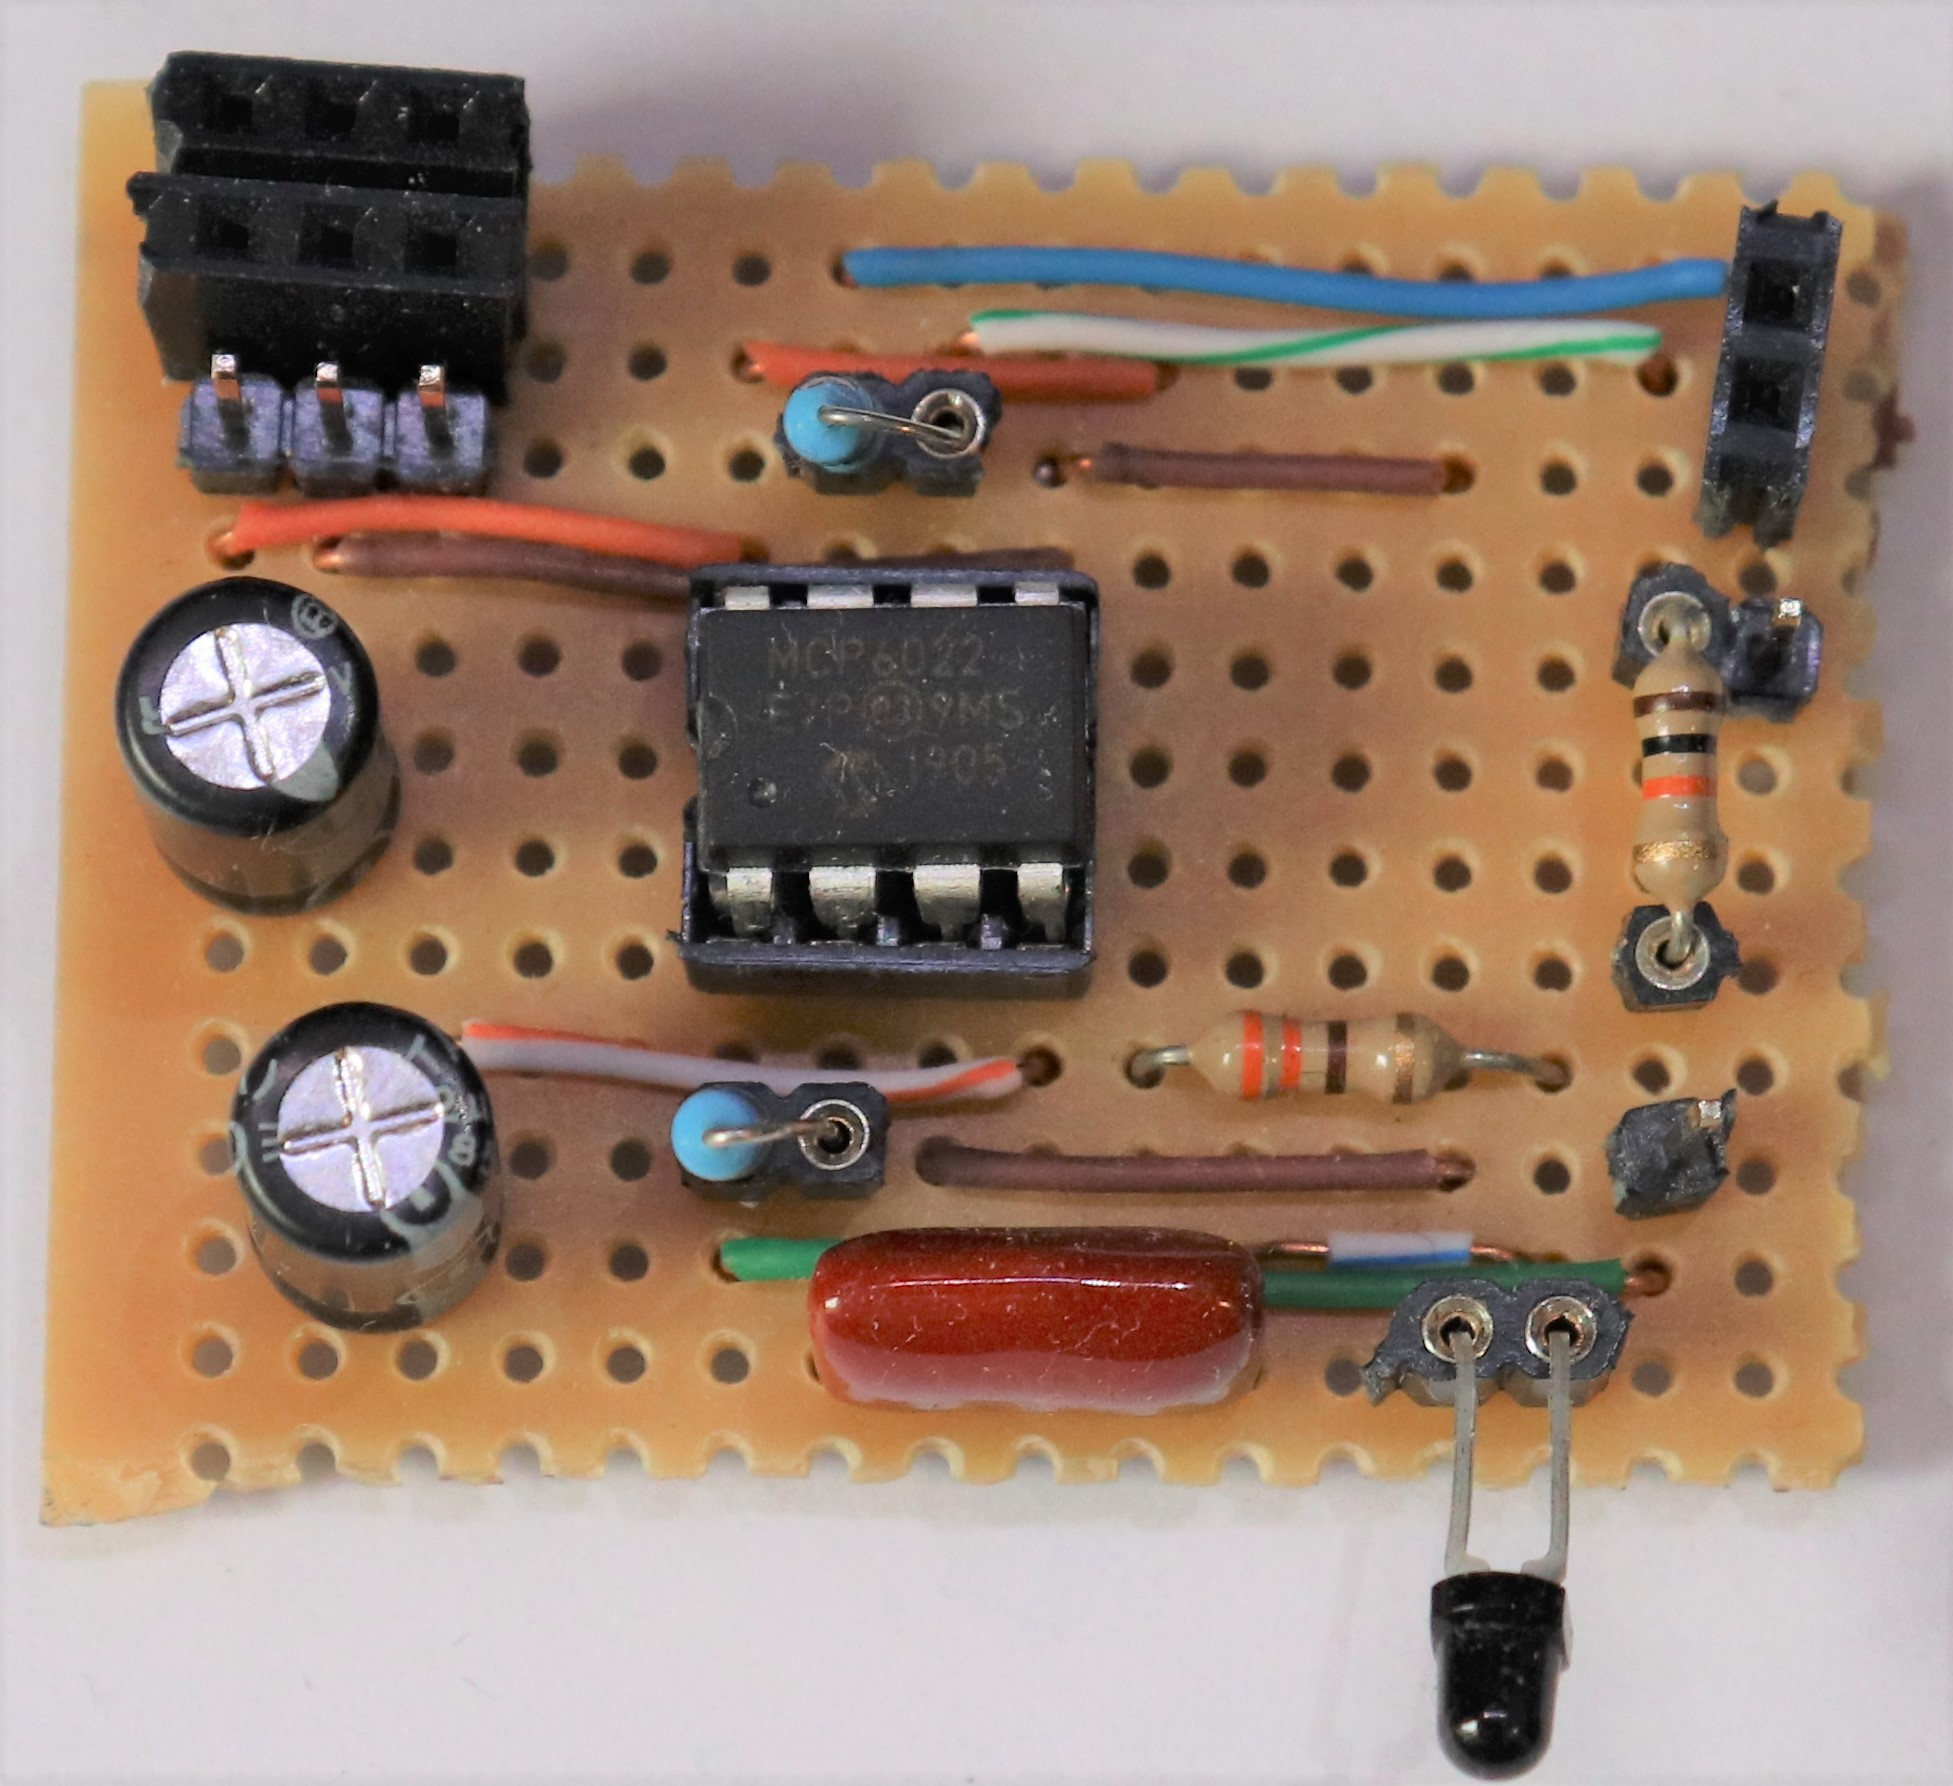
\includegraphics[width=.6\textwidth]{figures/modules/phototransistor_receiver.jpg}
	\caption{Phototransistor IR Detector Module}
	\label{fig:module_phototransistor_detector}
\end{figure}




%%%%%%%%%%%%%%%%%%%%%%%%%%%%%%%%%%%%%%%%%%%%%%%%%%%%%%%%%%%




\subsection{IR Receiver}
%Missing:
% - Schematic and explaination

\subsubsection{Functional Design}
The IR receiver is an 'all in one package' detector IC designed to detect the presence of a carrier signal in the IR light incident on the detector. The output of the module is high when no modulation is detected and pulled low when modulation is detected.

The module is designed to be powered by a 5V supply, however the output voltage has been clamped down to 3V to be compatible with the STM32 GPIO.

\subsubsection{Schematic}
Figure \ref{fig:schematic_voltage_clamp} below shows the schematic for the voltage clamp used to regulate the output of the TSOP382. The \href{https://www.vishay.com/docs/82491/tsop382.pdf}{datasheet} contains a block diagram (shown in figure \ref{fig:tsop382_block_diagram}) which gives a functional overview of the internal circuitry for this IC.


\begin{figure}[H]
	\centering
	\begin{minipage}{.5\textwidth}
		\centering
		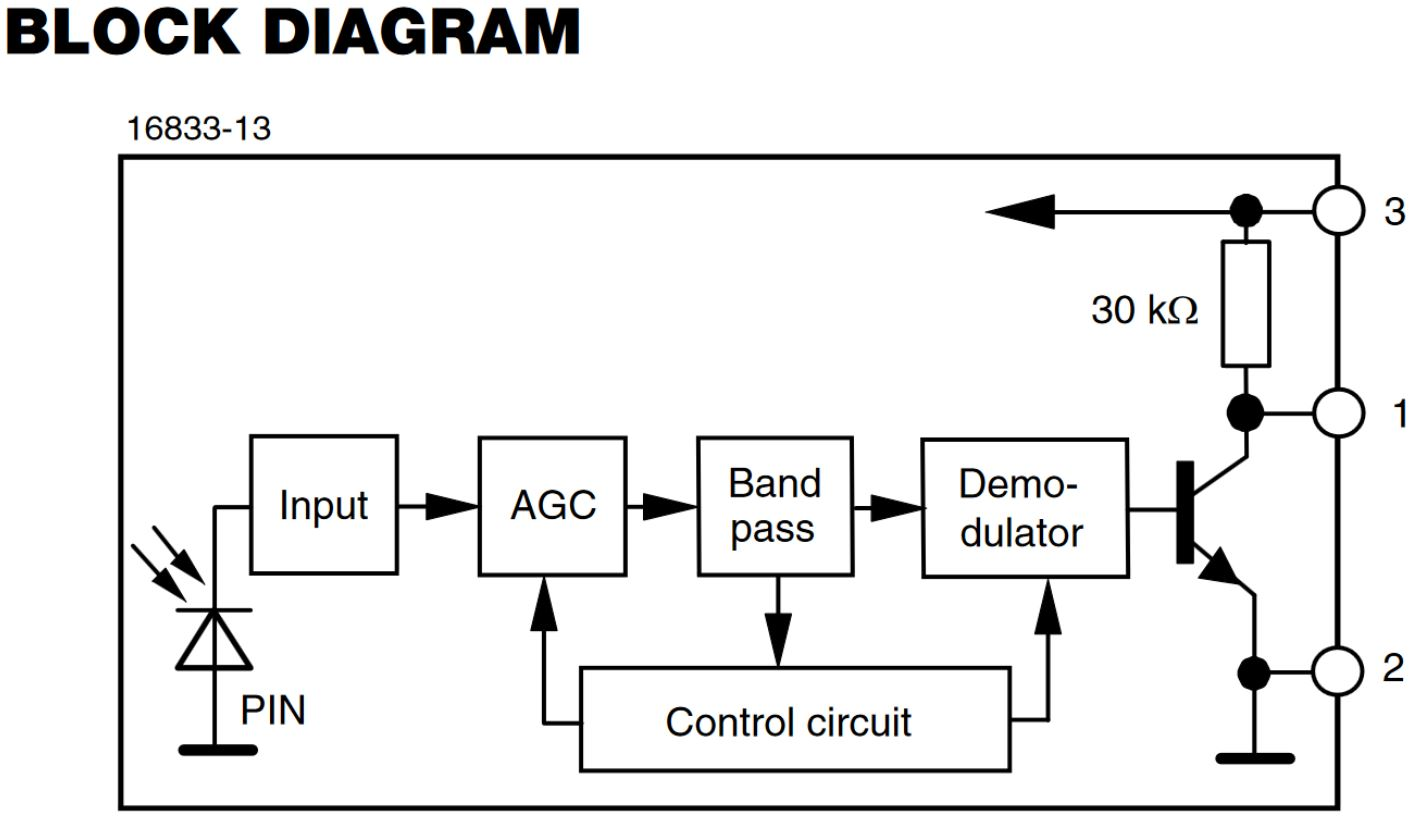
\includegraphics[width=.8\linewidth]{figures/design/TSOP382_block_diagram}
		\captionof{figure}{TSOP382 Functional Diagram}
		\label{fig:tsop382_block_diagram}
	\end{minipage}%
	\begin{minipage}{.5\textwidth}
		\centering
		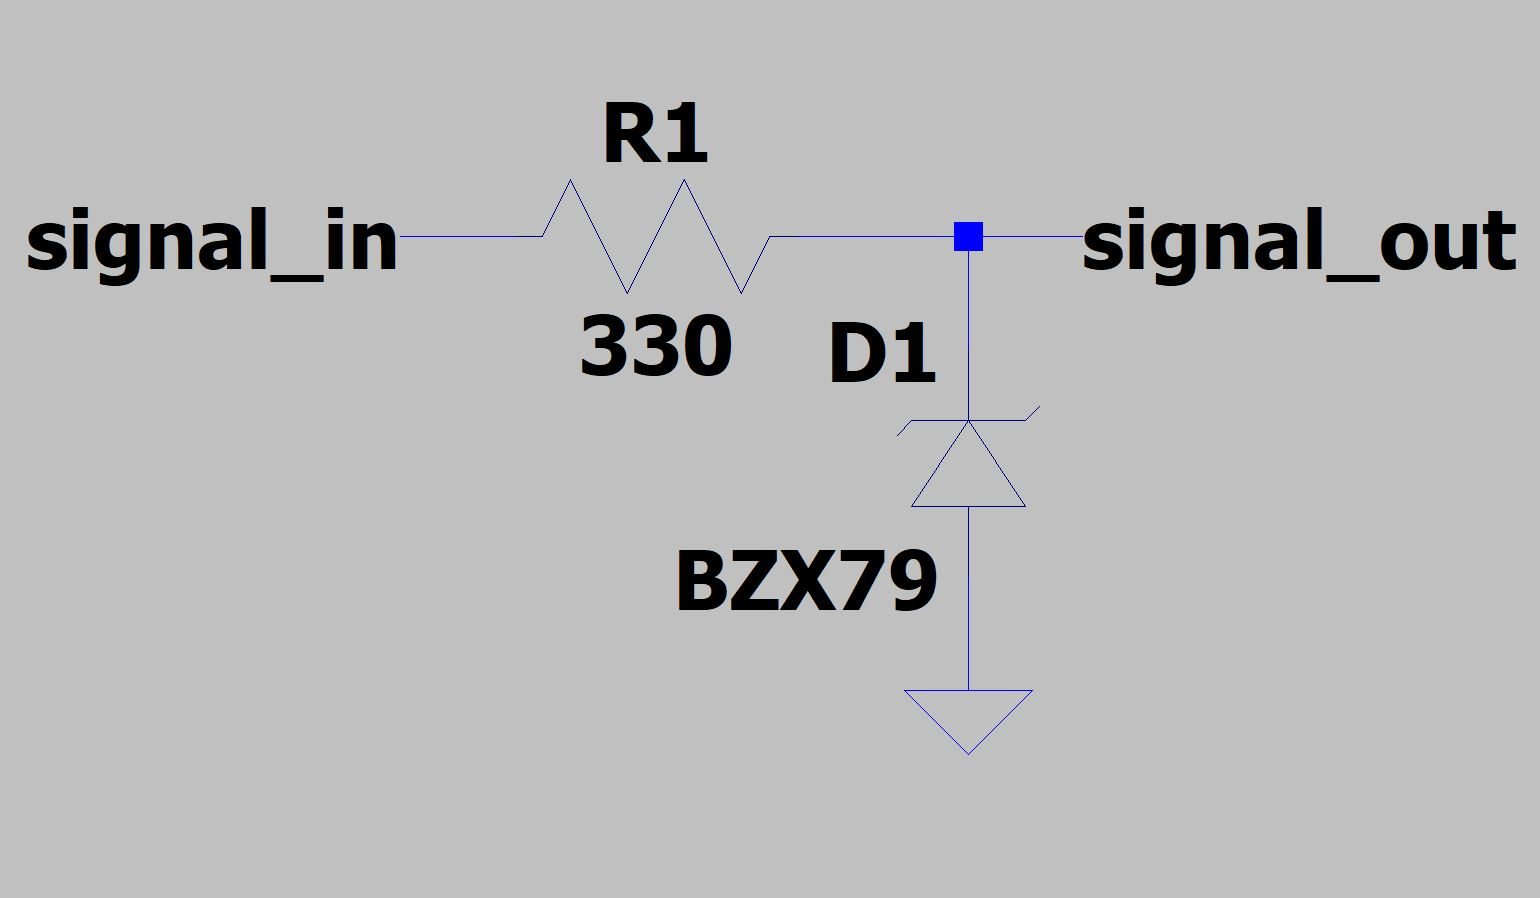
\includegraphics[width=.8\linewidth]{figures/design/over_voltage_protection}
		\captionof{figure}{Voltage Clamp}
		\label{fig:schematic_voltage_clamp}
	\end{minipage}
\end{figure}

\subsubsection{TSOP382}

The TSOP382 IR receiver was chosen due to it's low cost, availability and wide range of angles from which it can detect IR radiation. The purpose of this device is to act as a comparison with which to compare the photodiode and phototransistor IR detector modules.


\subsubsection{Module Realization}
The strip-board implementation of the module is shown in figure \ref{fig:module_ir_receiver} below.

\begin{figure}[H]
	\centering
	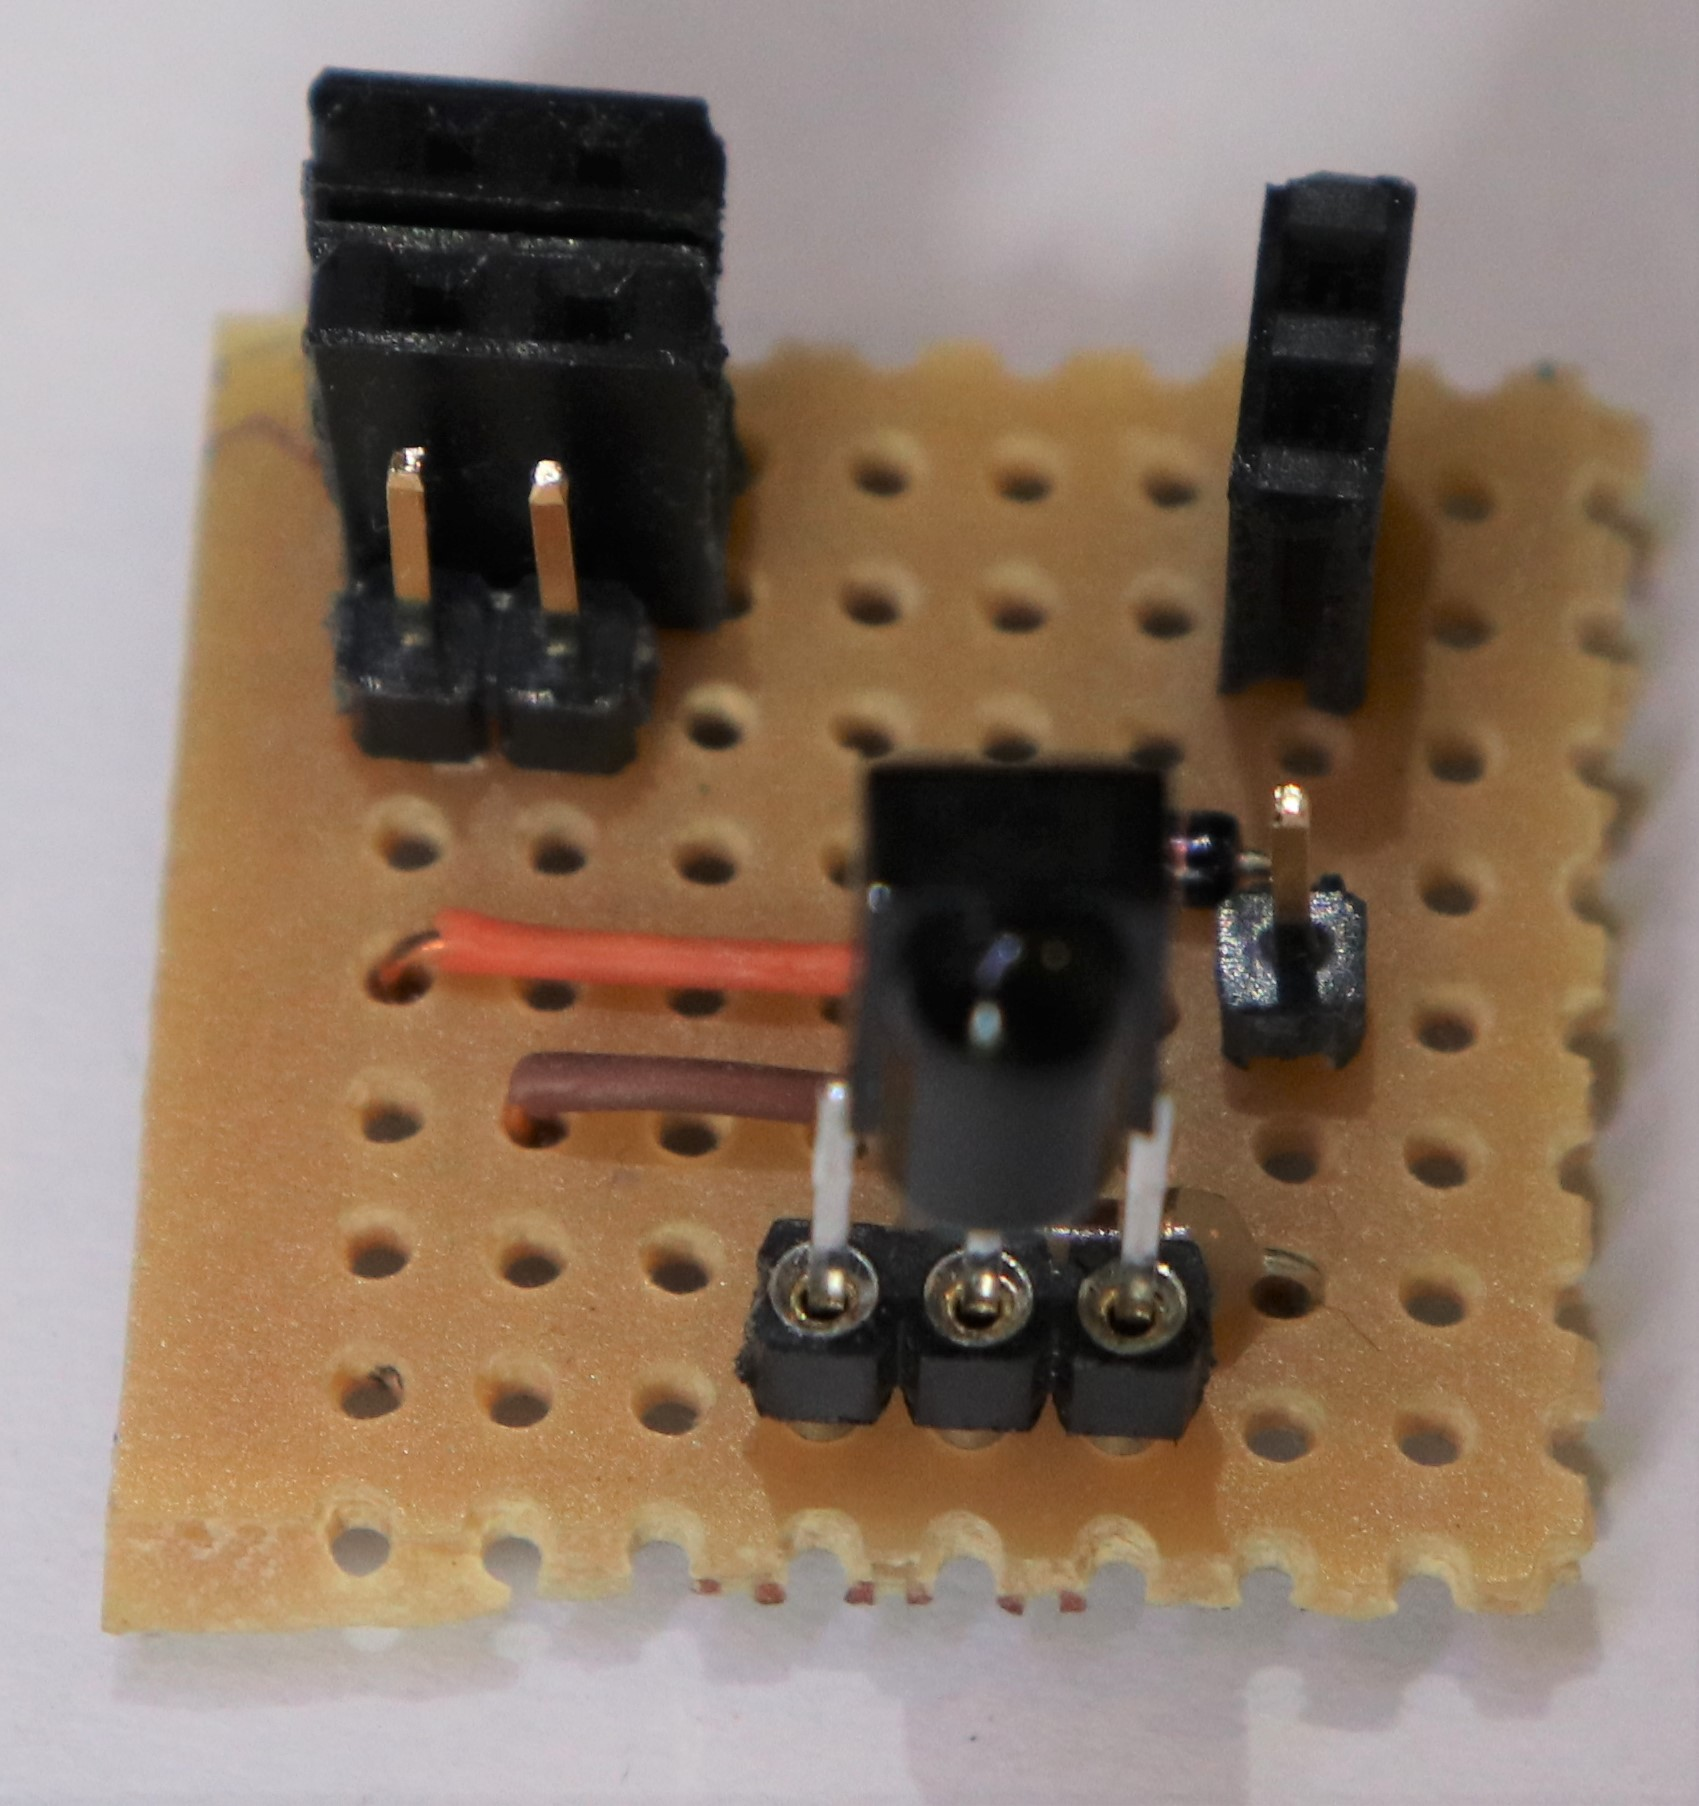
\includegraphics[width=.6\textwidth]{figures/modules/ir_receiver.jpg}
	\caption{IR Receiver Module}
	\label{fig:module_ir_receiver}
\end{figure}



%%%%%%%%%%%%%%%%%%%%%%%%%%%%%%%%%%%%%%%%%%%%%%%%%%%%%%%%%%%



\subsection{Signal Conditioning Module}
%Missing:
% - Choosing freq cut off and what is expected gain

The signal conditioning module can be broken into two stages. The first stage of the module performs filtering, this is prevent aliasing during the digital signal processing, which is caused by frequencies greater than half the sampling frequency being present in the sampled waveform. The second stage performs precision rectification, which is necessary to ensure a negative voltage is not placed on the input pin of the tone detector which has a tolerance range from 0V to 3.3V.

\begin{figure}[H]
	\centering
	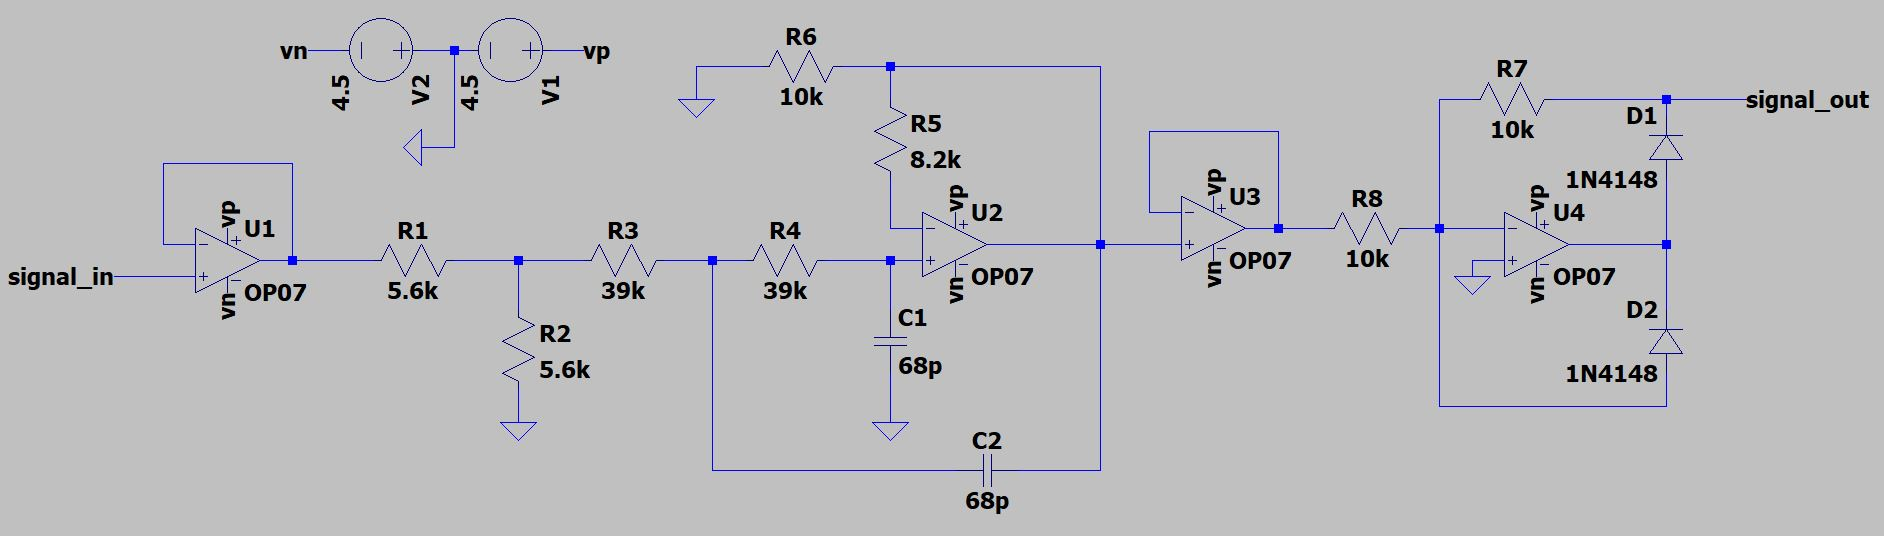
\includegraphics[width=\textwidth]{figures/design/filter_and_rectify}
	\caption{Signal Conditioning Module Schematic}
	\label{fig:schematic_filter_and_rectify}
\end{figure}

In most cases the incoming signal is a square wave which has formed due to the amplification stage of the detector module saturating at $\pm 4.5V$. To ensure the output signal is within the tolerance of the ADC, a voltage divider formed by R1 and R2 filter is place prior to the filter.

The filter circuit used is a second order voltage controlled voltage source (VCVS) active low pass filter in a Chebyshev configuration\footnote{0.5dB passband ripple}. The Chebyshev configuration was chosen because a sharp roll of is desired and because passband ripple will not affect the ability of the Goertzel filter to detect the target frequency. The component values where chosen in accordance to the filter design table found on page 274 of the book \textit{The art of electronics - 2nd Edition}\cite{Horowitz1995}.

The precision rectifier is also a circuit design taken from the book and can be found on page 188, it is an improved version of the basic precision rectifier because it reduces the output swing of the op-amp during operation\cite{Horowitz1995}.

\begin{figure}[H]
	\centering
	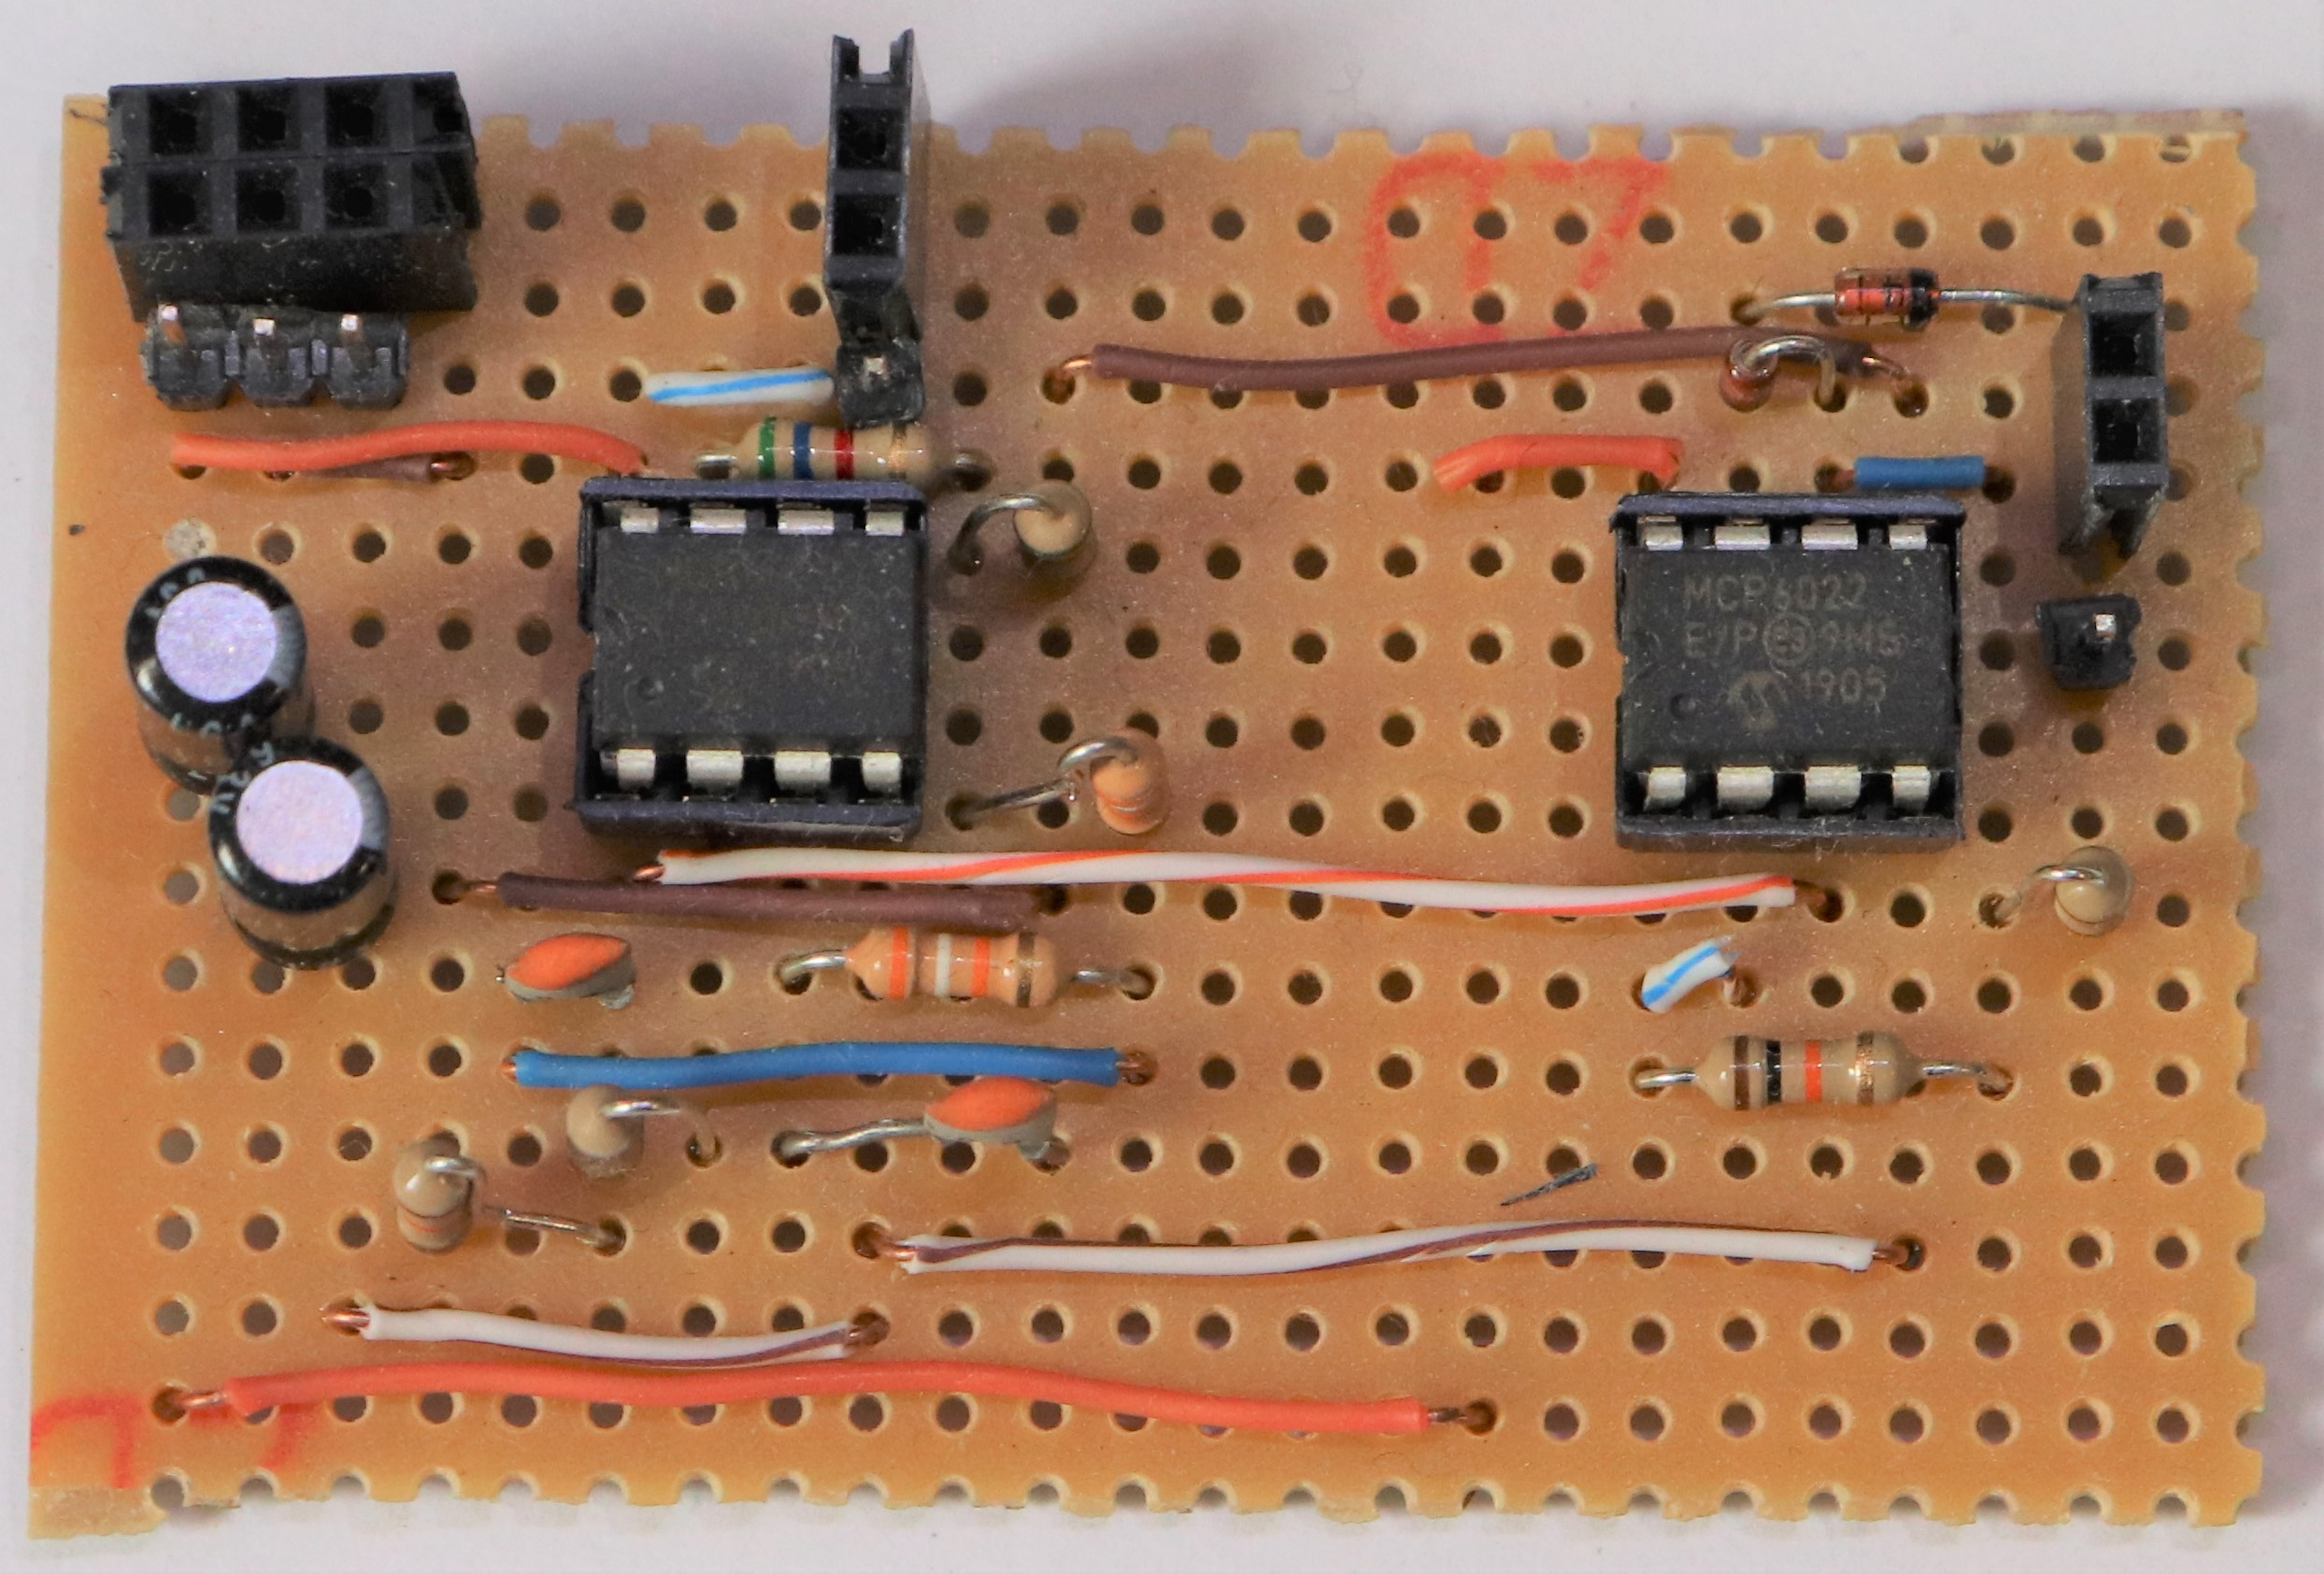
\includegraphics[width=.6\textwidth]{figures/modules/filtering_conditioning.jpg}
	\caption{Signal Conditioning Module}
	\label{fig:module_filtering_conditioning}
\end{figure}




%%%%%%%%%%%%%%%%%%%%%%%%%%%%%%%%%%%%%%%%%%%%%%%%%%%%%%%%%%%



\subsubsection{Filter Design}
%todo: desired freq cutoff and calculations


The desired cut-off frequency is \(f_{c} = 48kHz\), this defines the end of the passband\footnote{Unlike in the case of a Bessel filter, this is not necessarily the -3dB point}.

With reference to the schematic (figure \ref{fig:module_filtering_conditioning}), resistors and capacitors hold the following relations ships: \(R_3 = R_4 = R\) and \(C_1 = C_2 = C\).

According to the lookup table, to achieve a Chebyshev response, the following values should be used as the normalization factor and gain: \(f_n = 1.231\), \(K = 1.842\).

The gain is set by choosing $R_5$ and $R_6$ such that \(R_5 = (K - 1) \times R_6\) holds. The values of $R$ and $C$ are determined by the following equation


\[RC = \frac{1}{2\pi f_n f_c}\]

Substituting into the above equation we find $RC = 2.6935\times 10^{-6}$. It is recommended that the resistance value is between $10k$ and $100k$, the value of $39k\Omega$ was selected. The corresponding capacitance value is calculated to be $69pF$, and the E12 series capacitance value of $68pF$ was used.




%%%%%%%%%%%%%%%%%%%%%%%%%%%%%%%%%%%%%%%%%%%%%%%%%%%%%%%%%%%




\subsection{Tone Decoder Module}
%Missing:
% - Is a schematic worth the bother?

The tone decoder module's hardware consists of an STM32F051C6 breakout PCB which is mounted on a strip-board along with supporting circuity (external crystal and voltage regulation). In addition to the supporting circuitry, an over-voltage protection clamp (see figure \ref{fig:schematic_voltage_clamp}) was placed on pin 17 which is connected internally to PA7 which is configured as an analog input. Three signal LED's where wired to pins 18, 19 and 20 to act as status indicators.

The DSP algorithm is discussed in subsection \ref{tone_decoder_software} from the following section on software modules.


\begin{figure}[H]
	\centering
	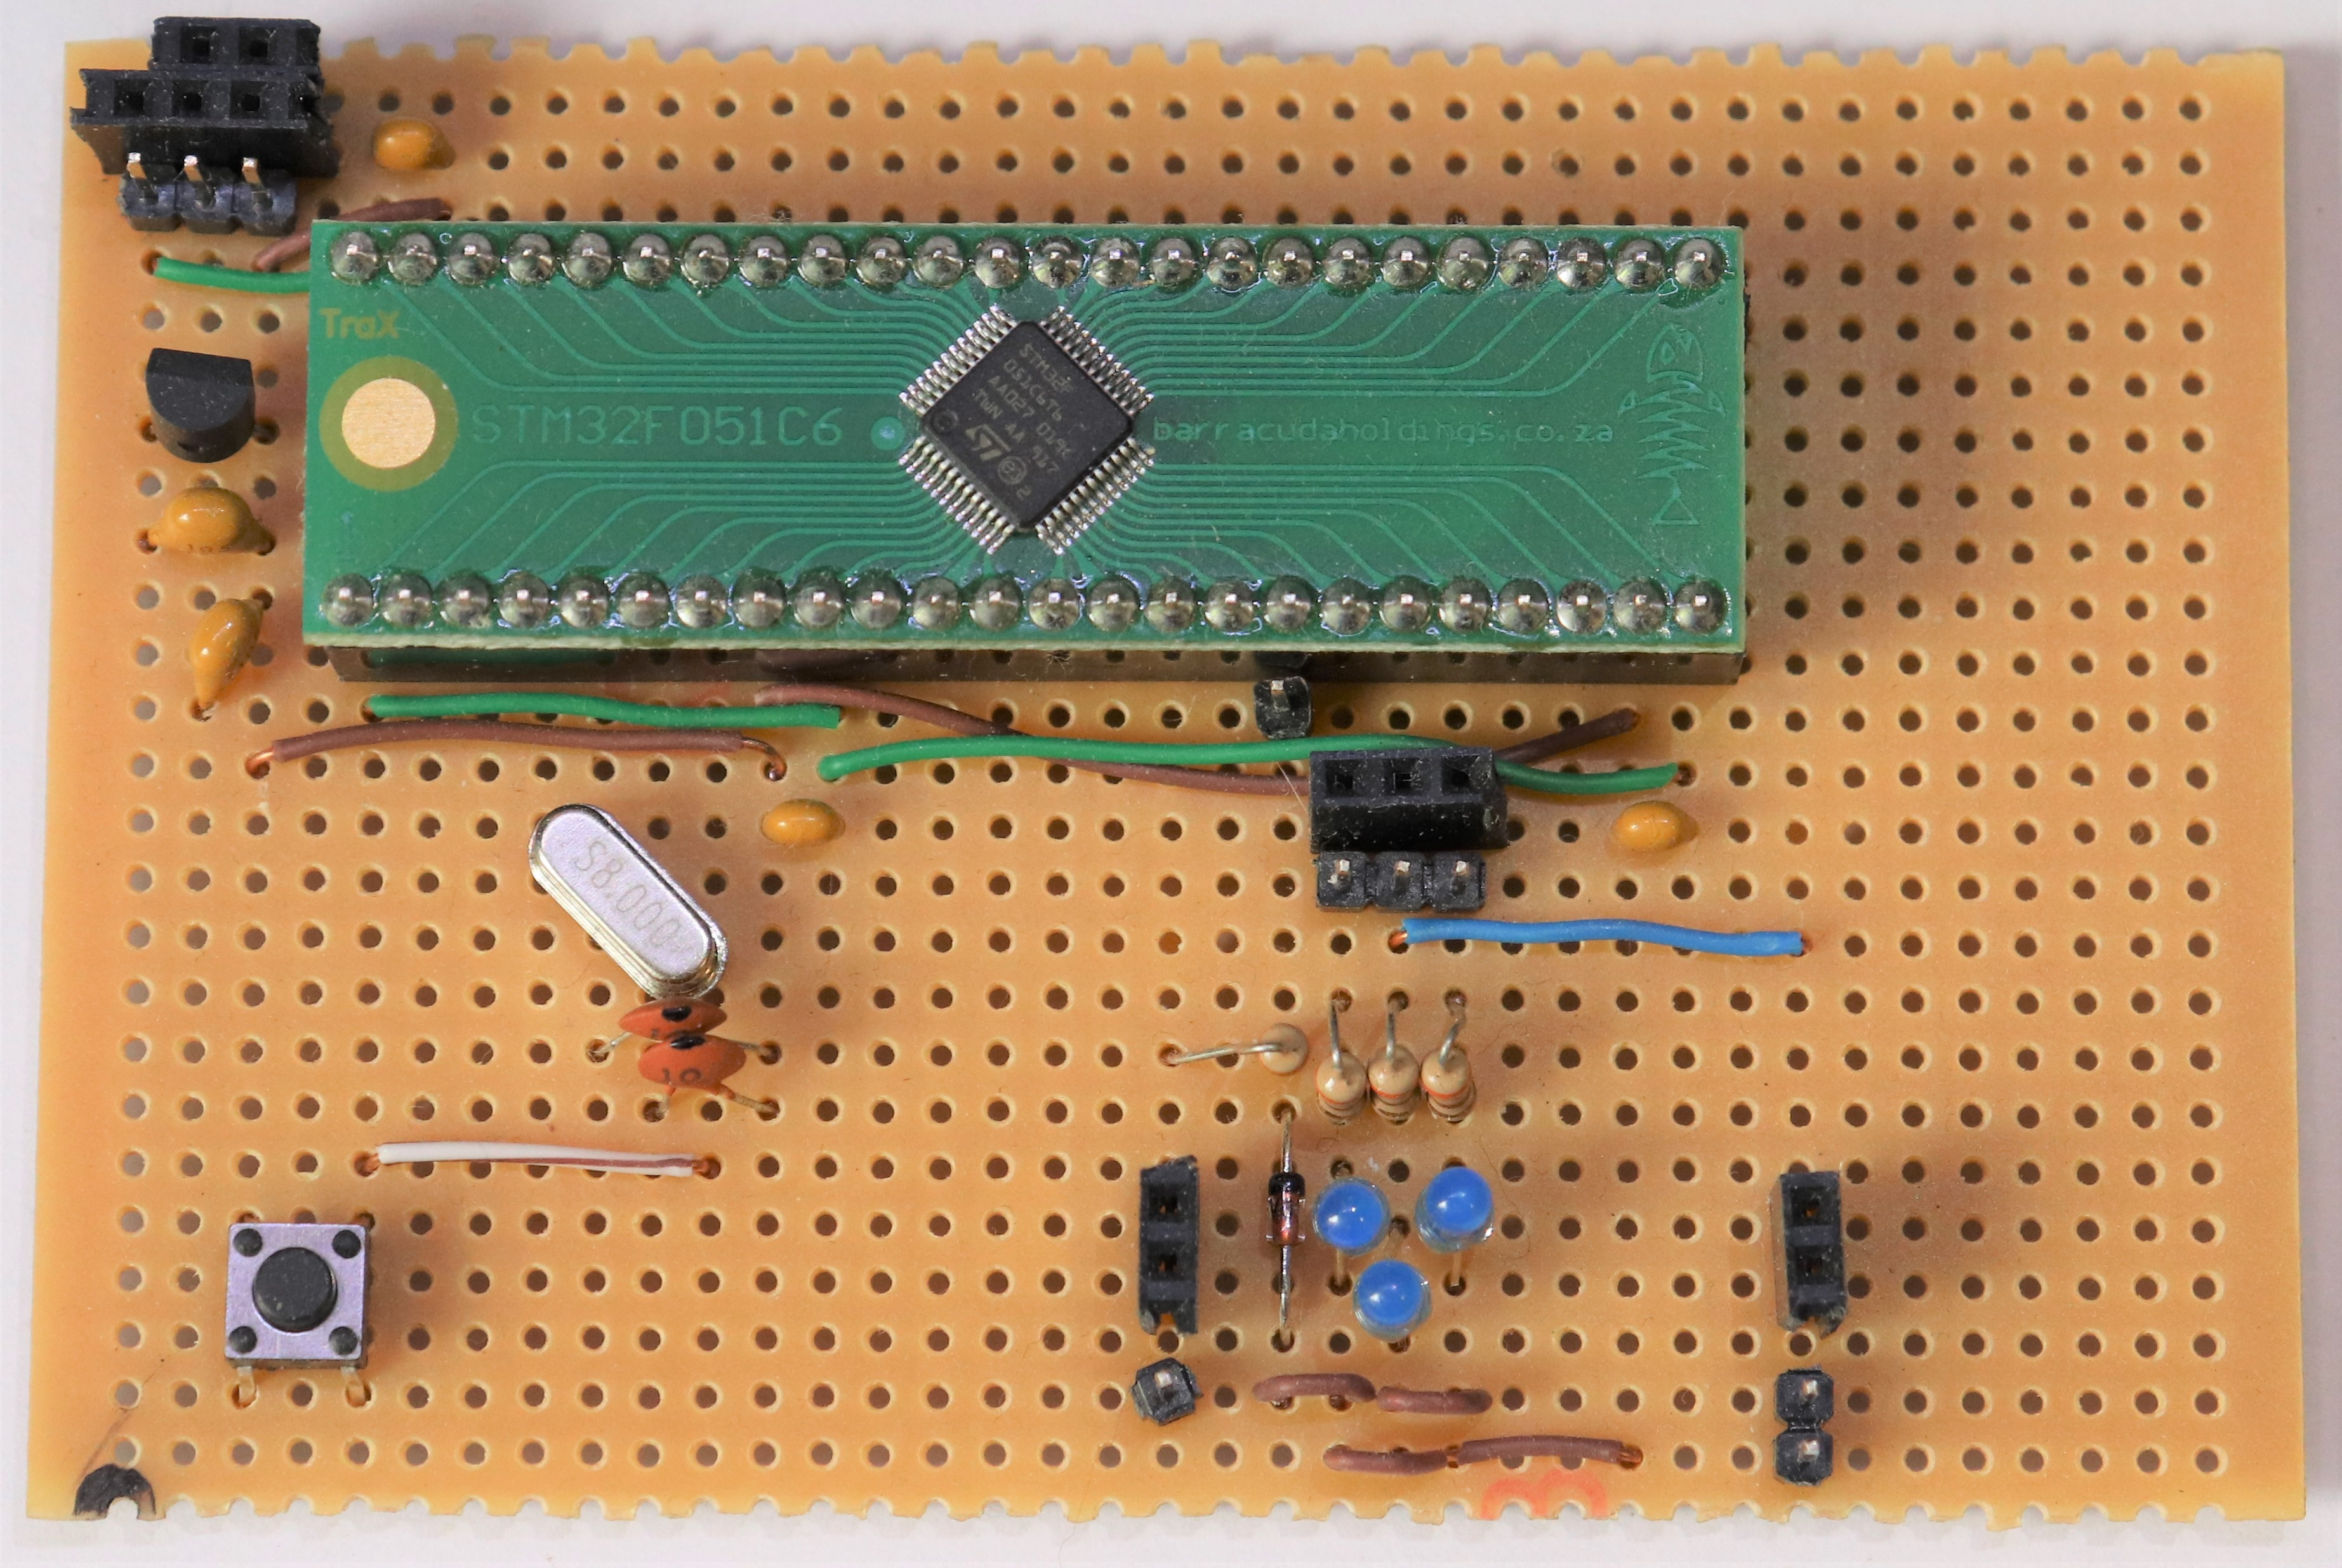
\includegraphics[width=.6\textwidth]{figures/modules/goertzel_filter.jpg}
	\caption{Tone Decoder Module}
	\label{fig:module_tone_decoder}
\end{figure}




%%%%%%%%%%%%%%%%%%%%%%%%%%%%%%%%%%%%%%%%%%%%%%%%%%%%%%%%%%%
%%%%%%%%%%%%%%%%%%%%%%%%%%%%%%%%%%%%%%%%%%%%%%%%%%%%%%%%%%%



\section{Software Design}

\subsection{Tone Decoder Software}
\label{tone_decoder_software}

In section \ref{sec:goertzel_implementation} the goertzel algorithm is given. The parameters k (the DFT frequency bin) and N (the number of samples per frequency bin coefficient calculation) determine the value of omega which in turn affects the value of 'cosval', 'sinval' and 'coeff'. The value of k is also affected by the ratio of the frequency of the k\textsuperscript{th} DFT frequency bin to the sampling frequency (f\textsubscript{sampling}).

The STM32F0 is designed to be low cost 32-bit microcontroller and utilizes the ARM Cortex-M0 CPU core. To reduce costs, this microcontroller does not contain any dedicated DSP peripherals nor does it contain any hardware dedicated to floating point arithmetic. Therefore careful consideration must be taken during design to optimize the performance of the goertzel filter implementation. The STM32F0 is equipped with several timers, a DMA peripheral and an advanced interrupt controller, these peripherals are indispensable for the implementation of the real-time digital filter. Figure \ref{fig:goertzel_functional_diagram} shows the functional blocks for the goertzel filter, the flow of data and clock signals.

\begin{figure}[H]
	\centering
	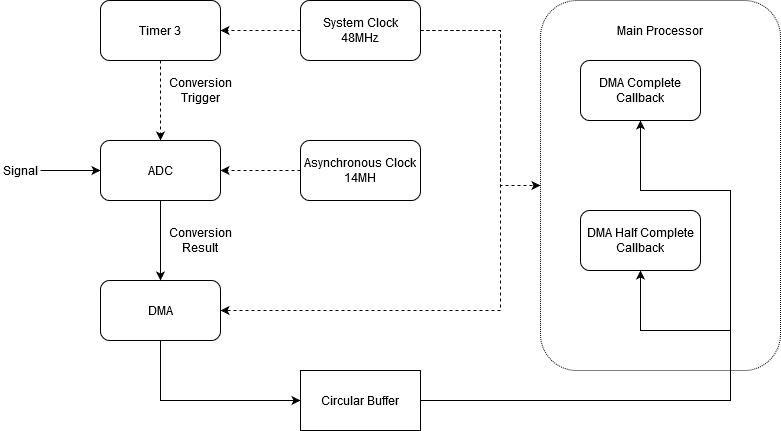
\includegraphics[width=.8\textwidth]{figures/design/goertzel_filter_functional.png}
	\caption{Goertzel Filter Functional Block Diagram}
	\label{fig:goertzel_functional_diagram}
\end{figure}

\subsubsection{Sampling Frequency Constraints}
\label{sec:sampling_frequency_constraints}
The sampling frequency determines the highest frequency that may be present in the sampled waveform before aliasing will occur. The higher the sampling rate, the wider the bandwidth of the goertzel filter. A higher sampling frequency also results in relaxed requirements for the antialiasing filter.

The sampling frequency is limited however by the speed of the microcontroller. This limitation influences the sampling frequency directly by acting as an upper bound to the rate at which the ADC can process and store each analog reading, however more critically, the sampling frequency is directly proportional to the number of samples that must be processed per period. Therefore it is necessary to keep the sampling frequency as low as possible.

\subsubsection{Filter Optimization}
\label{sec:filter_optimization_design}
As outlined at the beginning of this section, the most critical means of optimization for this filter is the full utilization of available peripherals. After reset, the main processor configures the timer, ADC and DMA to continuously sample the incoming signal and store the conversion results in a circular buffer. After this configuration, the main processor is freed from this process and all processing cycles are dedicated to processing the data being stored in the circular buffer.

The second means of optimization was realised after examination of the goertzel algorithm. By carefully engineering the configurable parameters in the goertzel algorithm (listing \ref{lst:goertzel_algorithm}) it is possible to reduce the computation time of the algorithm by removing the multiplication requirement for each new sample (line 13). This is achieved be choosing parameters that result in omega having a value of \(\frac{\pi}{2} + 2\pi m,\; m\epsilon \mathbb{Z}\) and as a consequence make 'cosval' and 'coeff' equal to zero.

It is important to note, this optimization does not improve the time complexity of the algorithm, in both cases the algorithm has a time complexity of O(N). However for real-time algorithms such as in the case of a goertzel filter, every possibly time saving is valuable and can be the difference between a working and failed implementation.

Line 4 of the algorithm provides the relationship between k, N and $\omega$

\begin{equation}
	\omega = \frac{2\pi * k}{N}
\end{equation}

Substituting \(\omega = \frac{\pi}{2} + 2\pi m,\; m\epsilon \mathbb{Z}\) and simplifying shows

\begin{equation}
\label{eqn:k_N_constraint}
	\frac{k}{N} = \frac{1+4m}{4},\; m\epsilon \mathbb{Z}
\end{equation}

If only integer values for k, N, $f_{sampling}$ and $f_{bin}$ are considered, line 3 of the algorithm provides the relationship between these parameters which may be expressed by the following equation

\begin{equation}
\label{eqn:k_N_and_fb_fs}
	\frac{k}{N} = \frac{f_{bin}}{f_{sampling}}
\end{equation}


Equation \ref{eqn:k_N_and_fb_fs} shows that the ratio of $f_{bin}$ to $f_{sampling}$ must be equal to that of k to N. This relationship reveals that the only realisable value for m is zero. Any value of m greater than zero requires a sampling frequency lower than the bin frequency which violates the Nyquist criteria and a negative value of m would require (for $f_{bin} \approx 36kHz$) a negative sampling frequency which is nonsensical. Therefore the final relationship between the ratios may be summarised in the following equation

\begin{equation}
\label{eqn:k_N_and_fb_fs_ratio}
\frac{k}{N} = \frac{f_{bin}}{f_{sampling}} = \frac{1}{4}
\end{equation}

Even after the above two means of optimizing the goertzel algorithm, the STM32F0 was not fast enough to process every sample. This is because even after optimizing the algorithm, it cannot processing incoming samples faster than the required 144kHz. The solution is to sample more than N samples per interrupt and drop the excess samples. This increases the amount of processing time per sample, but increases the latency between the filter's input and the output. This technique only works if the duration of modulation is much greater than the duration of samples dropped.

\subsubsection{Practical Implementation}

The desired bin frequency is 36kHz, according to equation \ref{eqn:k_N_and_fb_fs_ratio} this requires a sampling frequency of 144kHz. This is within the constraints set out in section \ref{sec:sampling_frequency_constraints}.

The ADC conversions are triggered by timer 3, a general purpose 16-bit timer. The timer accepts a pre-scalar and counter period value. The frequency of the timer's output and as a result the sampling frequency is given by \(f_{sampling} = \frac{f_{system\_clock}}{prescaler \times cperiod}\). Substituting our system clock frequency, desired sampling frequency and rearranging the equation we find the product of the pre-scalar and clock period values.

\[prescaler \times cperiod = \frac{48 \times 10^6}{144 \times 10^3} = 333.\dot{3}\]

The result, $333.\dot{3}$ cannot be formed as the product of two integer values, instead the closest integer value of 333 is used. Because this is well below the maximum value of the 16-bit counter period register, the pre-scalar is set to one. The resulting sampling frequency is $144.\dot{1}4\dot{4}$ kHz. Returning to equation \ref{eqn:k_N_and_fb_fs_ratio}, we see that we must choose $f_{bin} = 36.036$kHz to preserve the ratio required for optimization.

%todo: smitz trigger and such - did i do that yet??
The output of the Goertzel filter module is a digital state indicating the presence or absence of a 36kHz frequency. It was chosen to let a high output indicate the detection of the carrier frequency while a low output would indicate no detection.

A value of $6\times 10^{6}$ was selected as the threshold for the squared magnitude of the DFT bin's coefficient. A Schmitt-trigger was used to prevent oscillations while the squared magnitude of the coefficient is crossing this threshold. The output was configured to activate when the value exceeds the threshold by $2\times 10^{6}$ and deactivate when the value decreased by $2\times 10^{6}$ below the threshold.

\begin{figure}[H]
	\centering
	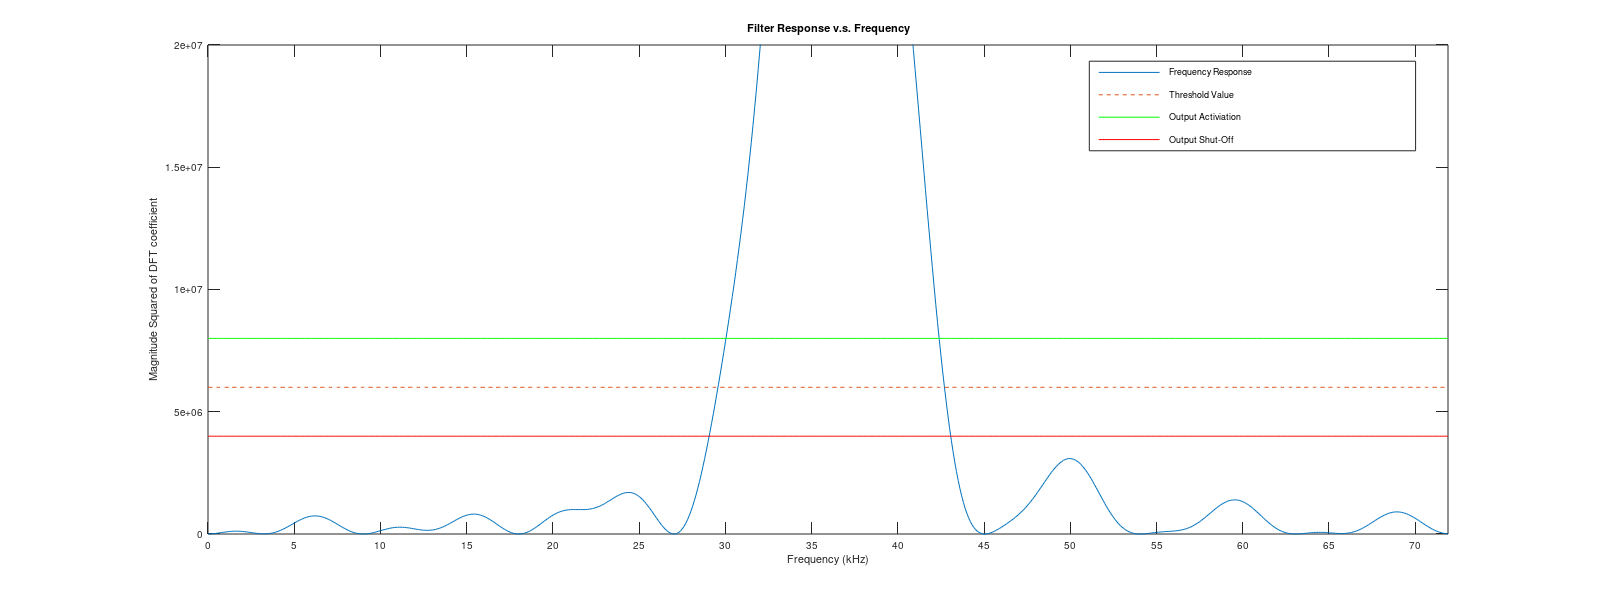
\includegraphics[width=.8\textwidth]{figures/design/schmit_simulation_wide.png}
	\caption{Schmitt Trigger Visualization}
	\label{fig:schmit_simulation_wide}
\end{figure}

Figure \ref{fig:schmit_simulation_wide} illustrates the activation and shut-off boundaries, based on the chosen threshold. The threshold and Schmitt-trigger values were chosen by inspecting the experimental results from the frequency response simulation results (see figure \ref{fig:goertzel_filter_response_simulated}) and selecting values which would allow sensitivity for input signals of differing amplitudes without triggering for side lobes of large amplitude signals.

%todo: ensure I mention improvements to this by using automatic gain control and therefore being able to raise the threshold value




%%%%%%%%%%%%%%%%%%%%%%%%%%%%%%%%%%%%%%%%%%%%%%%%%%%%%%%%%%%



\subsection{Tagger Software}

For the purposes of this investigation, a tagger needed to be created that can encode a gun ID and possibly some additional bits for other information. It was chosen to use a 16-bit packet size. In this initial implementation a single bit is reserved for error detection, however further development of this system might explore the use of hamming codes which would require an additional four bits to be reserved for error correction.

\subsubsection{Modified RC-5 Protocol}
The RC-5 protocol was used as the basis for the design of the modified transmission protocol. A detailed breakdown of the protocol is given in the literature review in section \ref{sec:rc_5_protocol}. In this modified version of the RC-5 protocol, the Manchester Encoding technique and bit-period timing specifications are preserved. However the structure of the bits transmitted has been modified and the period between messages was decreased.

\begin{figure}[H]
	\centering
	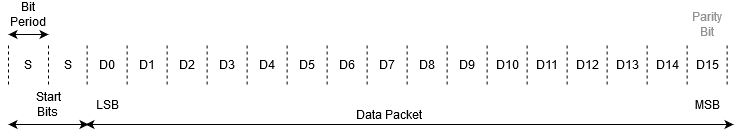
\includegraphics[width=0.8\linewidth]{figures/design/modified_rc5_protocol.png}
	\caption{Modified Bit Structure of RC-5 IR Protocol}
	\label{fig:modified_rc_5_protocol}
\end{figure}

Figure \ref{fig:modified_rc_5_protocol} shows the modified structure for a single transmission. The two start bits are preserved. Following this, the toggle bit, address bits and command bits have been merged into a single set of data bits with an additional 4 bits having been included to increase the number of bits to 16. In the modified protocol the bit order of has been reversed. It should be noted that data bit D15 is used for the parity checksum.

%todo: ref the experiement below
The original RC-5 protocol specifies a period of 114mS between transmissions, however this gap is longer than necessary and following the experiment performed in section \ref{label} it was determined that this period could be reduced to XXXmS.

\subsubsection{Realization}

The tagger software comprises a set of functions dedicated to the encoding of a 15-bit data packet. Implementation of the Manchester Encoding is done purely using timers and interrupts ensuring precise timing and freeing the main processor loop for handling lower priority tasks such as managing player data.

The following functions relating to the generation of a Manchester waveform on the pre-defined output GPIO pin were created

\begin{lstlisting}[style=cstyle, caption=Transmission Related Functions\label{transmission_related_functions}]
	uint8_t get_parity_15(uint16_t packet); //processes a 15-bit long data packet and returns the even parity
	uint32_t wrap_data_15(uint16_t data); //processes a 15-bit long data packet and returns 18-bit bitstream for transmission
	generate_manchester(uint32_t buffer, uint8_t num_bits); //starts Manchester encoded output generation on the pre-define GPIO based on the provided bitstream
\end{lstlisting}

Using one of the dedicated timer peripherals (timer 17) and interrupts for the process of generating the Manchester encoded output required the use of global variables to track the status of an on-going transmission. The following listing shows the global variables along with a brief descriptor comment.

\begin{lstlisting}[style=cstyle, caption=Transmission Status Tracking Variables\label{lst:transmission_status_tracking_variables}]
	volatile uint32_t bit_stream; //bit-stream to be transmitted
	volatile int bit_index; //index of bit currently being transmitted
	volatile int bit_num_transmit; //number of bits from bit-stream to transmit
	volatile int bit_period; //stores current bit period state (0 - first, 1 - second)
	volatile int fire_in_progress; //global indicator of a transmission in progress
	volatile int manchester_timeout_counter; //counts half bit-periods elapsed since last bit was transmitted
\end{lstlisting}

Using interrupts and global variables opens up the possibility for the data corruption to occur. Although the STM32F0 is inherently a serial processor, the main-loop process (responsible for, among other things, initiating transmissions) and the transmission process (the timer interrupt routine) from a high level execute as parallel processes. Figure \ref{fig:parallel_process_abstraction} illustrates how the operations during transmission may be abstracted as two parallel processes. Therefore it is critical to provide a mechanism to prevent one process from modifying any of the variable given in list \ref{lst:transmission_status_tracking_variables} while another process is using them.

\begin{figure}[H]
	\centering
	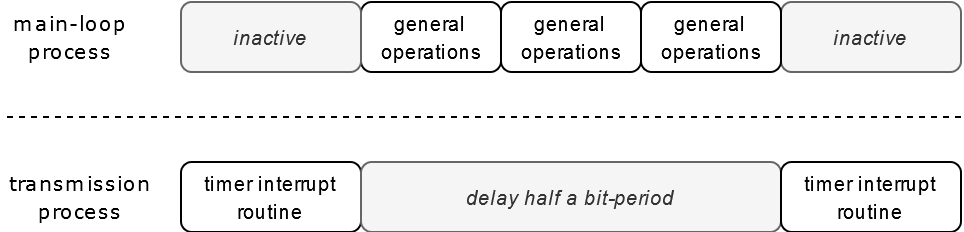
\includegraphics[width=0.8\linewidth]{figures/design/parallel_process_transmission.png}
	\caption{Parallel Process High-Level Abstraction}
	\label{fig:parallel_process_abstraction}
\end{figure}

The purpose of the variable \textit{fire\_in\_progress} is to operate as a synchronization lock. Priority is given to the interrupt process, therefore, in the implementation of the function \textit{generate\_manchester} there is a loop which stalls the processor until any current transmissions complete (see line 4, listing \ref{lst:generate_manchester_implementation}).

Finally, during the transmission process, the logic used to determine the pin state for the purpose of generating the Manchester waveform is given in line 8 of listing \ref{lst:manchester_generate_interrupt_routine}. The pin state for a given half bit-period can be determined as \[pin\_state = \overline{tx\_bit} \;\; \widehat{} \;\; bit\_period\] where tx\_bit is the value of the bit currently being transmitted and bit\_period is as defined in listing \ref{lst:transmission_status_tracking_variables} above.




%%%%%%%%%%%%%%%%%%%%%%%%%%%%%%%%%%%%%%%%%%%%%%%%%%%%%%%%%%%




\subsection{Target Software}

In laser tag it is optimal to have multiple IR detectors placed on various parts of the player. It is therefore important that the tagger software be extendable to process input from multiple input signals simultaneously. To achieve this, the input capture and output compare functions of the STM32 timer peripherals were used. For the purposes of this investigation, the system was developed to only capture a single incoming signal, however the process may be easily expanded to capture multiple incoming signals with little modification.

The target MCU software was separated into four independent processes, these are outlined in figure \ref{fig:target_software_overview} below.

\begin{figure}[H]
	\centering
	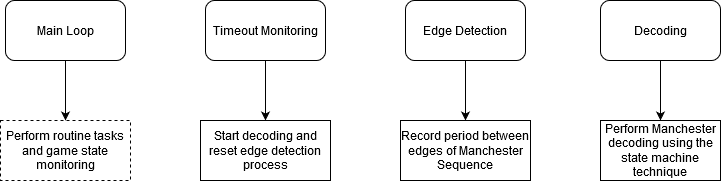
\includegraphics[width=0.8\linewidth]{figures/design/target_software_overview.png}
	\caption{Target MCU Processes}
	\label{fig:target_software_overview}
\end{figure}

The main loop process runs continually and may be used to perform routine tasks.

The edge detection is an interrupt based process which monitors continuously for any rising or falling edges on the input GPIO pin. Each edge is recorded as a time stamp which measures the period elapsed since the previous edge was detected. To reduce unnecessary computation, this value was stored in \textit{ticks} rather than converted into seconds.

The timeout monitoring process is executed by via an interrupt when the output compare register matches the timer's count value. Each time an edge is registered by the edge detection process, the output compare register value is adjusted to allow up to one timeout period before the interrupt is triggered.

The decoding process is an interrupt triggered processes which may also be triggered by software (when the maximum number of edges are recorded). This process decodes the time stamps recorded by the edge detection process and returns the recovered data. The decoding process uses the state machine approach illustrated in figure \ref{fig:manchesterdecodingfsm}.

During the decoding process, the edge detection process responsible for triggering the process is prevented from recording any further edges until the decoding is finished.

\subsubsection{Decoding Strategy}

The state machine approach does not specify an end of transmission condition, therefore it is necessary to define one. It is not possible to simply count the cumulative number of bits as the input capture stage and decoding stages are independent. Therefore a timeout timer will be implemented to trigger the decoding and reset the \textit{array of edge time} differences. In addition to a timeout a maximum number of edges is defined which will also trigger the start of a decoding sequence and reset the state machine.

The timeout period was chosen to be a length of two bit-periods, this was chosen because future inclusion of hamming codes would allow for the correction of a single flipped or missing bit. The timeout period of 3.556ms must be converted into a number of ticks before being used by the output compare functionality of the timer.

\[TIMEOUT\_TICKS = f_{timer} \times T_{timeout} = 8 \times 10^6 \times 3.556 \times 10^{-3} = 28448\]

The maximum number of edges in a valid message occurs when all 16-bits are 1's which results in a Manchester sequence containing 36 edges. Therefore the edge detection process will automatically begin the decoding process if 36 edges are recorded.

The implementation of the Manchester decoding algorithm may be found in the appendix, listing \ref{lst:decode_manchester_implementation}. Decoding requires a time period which defines the difference between a long and short period. This is the \textit{THRESHOLD\_TICKS} constant, in addition a second constant \textit{BITMISS\_TICKS} was defined and is used as a threshold to determine if a bit in the message has been was undetected.









